%Dokumentklasse
\documentclass[a4paper,10pt]{scrreprt}
\usepackage[left= 2.5cm,right = 2cm, bottom = 4 cm]{geometry}
\usepackage[onehalfspacing]{setspace}
% ============= Packages =============

% Dokumentinformationen
\usepackage[
	pdftitle={Titel der Abschlussarbeit},
	pdfsubject={},
	pdfauthor={Euer Name},
	pdfkeywords={},	
	%Links nicht einrahmen
	hidelinks,
	breaklinks
]{hyperref}

\urlstyle{same}


% Standard Packages
\usepackage[utf8]{inputenc}
\usepackage[ngerman]{babel}
%\usepackage[T1]{fontenc}
\usepackage{fontspec}
\defaultfontfeatures{Mapping=text-text}
\setsansfont{Verdana}
\renewcommand*{\familydefault}{\sfdefault}
%\linespread{1.25}
\usepackage{graphicx, subfig}
\graphicspath{{img/}}
\usepackage{fancyhdr}
\usepackage{lmodern}
\usepackage{color}
\usepackage{hyperref}
\usepackage{float}
% zusätzliche Schriftzeichen der American Mathematical Society
\usepackage{amsfonts}
\usepackage{amsmath}

%nicht einrücken nach Absatz
%\setlength{\parindent}{0pt}


% ============= Kopf- und Fußzeile =============
\pagestyle{fancy}
%
\lhead{}
\chead{}
\rhead{\slshape \leftmark}
%%
\lfoot{}
\cfoot{\thepage}
\rfoot{}
%%
\renewcommand{\headrulewidth}{0.4pt}
\renewcommand{\footrulewidth}{0pt}

% ============= Package Einstellungen & Sonstiges ============= 
%Besondere Trennungen
\hyphenation{De-zi-mal-tren-nung}

\setlength{\parindent}{0pt}


% ============= Dokumentbeginn =============

\begin{document}
%Seiten ohne Kopf- und Fußzeile sowie Seitenzahl
\pagestyle{empty}

\begin{center}
\begin{tabular}{p{\textwidth}}


%\begin{center}
%\includegraphics[scale=0.5]{img/logos.jpg}
%\end{center}


\\

\begin{center}
\LARGE{\textsc{
Entwicklung einer Webanwendung (Workshoppy) zur
Durchführung von Workshops in Echtzeit\\
}}
\end{center}

\\

\begin{center}
\textbf{\Large{Abschlussarbeit}}
\end{center}

\begin{center}
zur Erlangung des akademischen Grades\par
Bachelor of Science (B.Sc)
\end{center}

\begin{center}
an der\par
\end{center}

\begin{center}
\large{Hochschule für Technik und Wirtschaft Berlin\par
Fachbereich 4\par
Studiengang Angewandte Informatik \\}
\end{center}

\begin{center}
vorgelegt von
\end{center}

\begin{center}
\large{\textbf{Alongkorn Kiatmontri}} \\
\end{center}

\begin{center}
\large{(eingereicht am )}
\end{center}

\\

\\

\begin{center}
\begin{tabular}{lll}
\textbf{Erstprüfer:} & & Herr Prof. Jung, Th.\\
\textbf{Zweitprüfer:} & & Herr Andreas Flack (LB)\\
\end{tabular}
\end{center}

\end{tabular}
\end{center}

\addsec{Eidesstattliche Erklärung}
\label{erklaerung}

Hiermit versichere ich, die vorliegende Abschlussarbeit selbstständig und nur unter Verwendung der von mir angegebenen Quellen und Hilfsmittel verfasst zu haben. Sowohl inhaltlich als auch wörtlich entnommene Inhalte wurden als solche kenntlich gemacht. Die Arbeit hat in dieser oder vergleichbarer Form noch keinem anderem Prüfungsgremium vorgelegen.\\
\\[1.5cm]
Datum:	\hrulefill\enspace Unterschrift: \hrulefill
\\[3.5cm]

\newpage
\addsec{Danksagungen}
\label{danksagungen}




\addsec{Zusammenfassung / Abstract}
\label{sec:zusammenfassung}


\minisec{Abstract}
\label{abstract}


% Beendet eine Seite und erzwingt auf den nachfolgenden Seiten die Ausgabe aller Gleitobjekte (z.B. Abbildungen), die bislang definiert, aber noch nicht ausgegeben wurden. Dieser Befehl fügt, falls nötig, eine leere Seite ein, sodaß die nächste Seite nach den Gleitobjekten eine ungerade Seitennummer hat. 
\cleardoubleoddpage

% pagestyle für gesamtes Dokument aktivieren
\pagestyle{fancy}

%Inhaltsverzeichnis
\tableofcontents

%Verzeichnis aller Bilder
\listoffigures

%Verzeichnis aller Tabellen
\listoftables

\chapter{Einleitung}
\label{sec:einleitung}
Im ersten Kapitelabschnitt der Bachelorarbeit, wird auf die Motivation und die Zielsetzung eingegangen. Zusätzlich wird ein Überblick über den Aufbau der Arbeit aufgezeigt.

\section{Motivation}
\label{sec:motivation}
Beim Suchen und Finden von Lösungen, ungewöhnlichen Geschäftsideen, Innovationen oder um einzelne Projekte erfolgreicher zu machen, bereichert viele Menschen der Begriff Kreativität. Um die Kreativität zu fördern, braucht es Kreativitätstechniken, die dabei helfen, Ideen zu generieren und Einfälle zu sammeln.\bigskip

Der Klassiker und eine der bekanntesten unter allen Kreativitätstechniken ist das klassische Brainstorming. Sie wurde vom Amerikaner Alex Faickney Osborn erfunden und von Charles Hutchison Clark zur Ideenfindung innerhalb von Gruppen weiterentwickelt. 
(vgl. \cite{Ben.o.J.}) \glqq Er benannte das Brainstorming nach der Idee dieser Methode, nämlich using the brain to storm a problem (wörtlich: Das Gehirn verwenden zum Sturm auf ein Problem).\grqq{} \cite{Pas2012}\bigskip

Die Kreativitätstechnik Brainstorming gilt als eine der beliebtesten Methoden zur Ideenfindung und -sammlung neuer Geschäftsideen, Ideen für ein Projekt/Produkt oder auch zu einer vorhandenen bzw. gegebenen Problemstellung.\bigskip

Ziel des Brainstormings ist es, Denkblockaden auf der Suche nach neuen Ideen zu beenden. Diese Kreativitätstechnik wird häufig in Seminaren und Workshops angewendet, um die Gruppenarbeit effektiver und effizienter zu gestalten. Bei einer Brainstorming-Sitzung in einem Workshop kann jeder Teilnehmer auf die Ideen des anderen aufbauen und anknüpfen. Dadurch werden die Teilnehmer gegenseitig durch Ihre Ideen zu neuen Ideen angeregt, wodurch mehr Ergebnisse, als tatsächlich gebraucht, produziert werden.\bigskip

Eine häufig angewendete Methodik für die Ausarbeitung des Brainstormings in den Workshops ist es, sich Karteikarten oder Notizzettel zu nehmen, seine Ideen und Gedanken darauf zu schreiben und an eine Pinnwand (Flipchart, Whiteboard) anzubringen. Haben alle Teilnehmer Ihre Karteikarten an der Pinnwand angebracht, wird anschließend analysiert und darüber diskutiert. Am Ende der Besprechung werden die gesammelten Daten bewertet und anschließend von dem Moderator dokumentiert. Mit herkömmlichen analogen Workshops bedeutet das für den Moderator, dass er die Karteikarten auf der Pinnwand abtippen oder abfotografieren muss, um eine Dokumentation erstellen zu können. Da wir uns heutzutage in einem digitalen Zeitalter befinden und uns dieser neuen Welt nicht mehr entziehen können, gilt es, diesen Wandel als Chance zu begreifen, solche analogen Workshops zu digitalisieren, um dem Moderator eine Möglichkeit anzubieten, die Daten digital zusammenzufassen.

\section{Zielsetzung und Aufbau der Arbeit}
\label{subsec:zielsetzung}
Im Rahmen dieser Bachelorarbeit soll eine dynamische Webanwendung (Workshoppy) zur Durchführung von Workshops in Echtzeit entwickelt werden, die das klassische Brainstorming digitalisieren und effektiver machen soll. Die Webanwendung soll künftig in den Workshops genutzt werden und muss die Funktionen bieten, welche mehrere Personen (Teilnehmer) über Ihre Endgeräte (Smartphone, Laptop oder Tablet) ihre Ideen abgeben können. Dabei werden die eingebrachten Ideen der Teilnehmer in Echtzeit auf einer großen Leinwand (Beamer) präsentiert. Der Moderator soll anschließend die Möglichkeit erhalten, die Ergebnisse digital zusammenzufassen. Die Zusammenfassung soll auch als PDF-Datei exportiert werden können. Bei der Konzeption der Webanwendung ist zu beachten, dass eine benutzerfreundliche Darstellung für die Anwender gewährleistet ist.\bigskip

Die vorliegende Arbeit ist wie folgt aufgebaut: Das Kapitel \textbf{\ref{sec:grundlagen}} stellt vorab ein Überblick über einige grundlegende Begriffe vor. Der Begriff Responsive Webdesign, AJAX-Technologie und Rich Internet Applications (RIA) werden besprochen. Anschließend wird der Thin Client und Thick Client beschrieben. Das Kapitel \textbf{\ref{sec:analyse}} beschäftigt sich zunächst mit dem Stand der Technik. Die Anforderung zur Webanwendung wird dabei analysiert und konzipiert. In diesem Kapitel werden vor allem die funktionale, nicht-funktionale Anforderungen sowie die Muss- und Kann- Anforderungen ermittelt. Aufbauend auf den Ergebnissen der Anforderungsanalyse erfolgt in Kapitel \textbf{\ref{sec:design}} eine ausführliche Beschreibung über den Entwurf der Benutzeroberfläche (GUI) der Webanwendung. Danach wird das Design der GUI entworfen. Im Kapitel \textbf{\ref{sec:implementierung}} wird zunächst die zu verwendenden Webentwicklungswerkzeuge vorgestellt. Anschließend beschäftigt sich dieses Kapitel hauptsächlich mit der Implementierung der Webanwendung. Nach der Implementierung wird das Endergebnis im Kapitel \textbf{\ref{sec:bewertung}} anhand eines Fragebogens bewertet. Zum Schluss wird es im Kapitel \textbf{\ref{sec:schluss}} die erarbeiteten Ergebnisse zusammengefasst, sowie Ideen für zukünftigen Erweiterungen der entwickelten Webanwendung diskutiert.


\chapter{Grundlagen}
\label{sec:grundlagen}
Dieses Kapitel behandelt die für diese Arbeit nötigen Grundlagen. Zunächst wird ein Überblick über grundlegende Begriffe vorgestellt. Das Responsive Webdesign und einige Merkmale für eine responsive Webseite in Bezug auf die zu entwickelnde Webanwendung werden erläutert. Dann werden das Web 2.0 und der entstandene Ausdruck \textit{Rich Internet Application} beschrieben. Anschließend gibt es die Unterschiede zwischen Thin Client und Thick Client.

\section{Grundlegende Begriffe}
\label{sec:grundlegende begriffe}

\subsection{Workshop}
\label{sec:workshop}
Workshop\footnote{bedeutet so viel wie \glqq Arbeitskreis oder -gruppe\grqq{} .} ist eine Veranstaltung, bei der sich eine bestimmte Anzahl von Personen teilnimmt, um außerhalb der Routinearbeit Fragen, Probleme und Themen zu bearbeiten. Jeder Workshop wird von einem Moderator geleitet. Bei größeren Gruppen (mehr als 15 Teilnehmer) ist der Einsatz von weiteren Moderatoren zu empfehlen. Die Teilnehmer handeln es sich in der Regel um Spezialisten oder Betroffene, die Ihr Fachwissen zu der behandelten Aufgabe einfließen lassen. Das Ziel ist dabei: Lösungsvorschläge für Aufgaben- oder Problemstellung zu generieren und Maßnahmenplan für die Umsetzung zu entwickeln.
\\

Der Moderator ist der aktiver Dienstleister der Gruppe. Er ist für die Vorbereitung sowie Organisation verantwortlich und soll die Gruppe am Ende zum Ziel führen. Seine Aufgaben bestehen unter anderem, Fragestellung gezielt zu formulieren, den Ablaufplan zu erstellen, Denkprozesse anzuleiten, Zeitplan einzuhalten und Ergebnisse zu dokumentieren. Er muss außerdem die stille Teilnehmer aktivieren sowie die dominante bremsen und darauf achten, dass die Gruppe bei Diskussionsrunden das Ziel nicht aus den Augen verliert. 
\\

Nach Ansicht des Autors \cite{Boh2016} können Workshops in folgenden Projektphasen eingesetzt werden:

\begin{itemize} 
\item Kick-Off-Veranstaltung
\item Projektplanung-Prozess
\item Problemlösung
\item Entscheidungsfindung
\item Informationsaustausch
\item Teamentwicklung
\item Scrum
\item Projektabschluss
\end{itemize}

Die Gestaltung von Workshops spielt bei der Qualität der Ergebnisse eine große Rolle. Bei einem unstrukturierten Workshop kann dazu führen, dass er keine Motivation bei den Teilnehmer erregt, um sich an dem Workshop einzubringen und Ergebnisse zu erarbeiten. Um dagegen vorzugehen, können der Moderator je nach Dauer des Workshops folgenden kreative Workshop-Methoden anwenden, um Workshops effektiv und interaktiv zu gestalten:

\begin{itemize} 
\item World Cafe
\item Open Space
\item Six Thinking Hats
\item Fishbowl
\item Lego Serious Play
\end{itemize}

Die genauen Beschreibungen zu den oben genannten Workshop-Methoden können im Blogpost von \cite{Cho2018} verfolgt werden.
\\

Wenn es darum geht, neue Ideen für Problemlösung, neue Produkten, neue Geschäftsideen oder Innovationen zu erzeugen, werden Kreativitätstechniken eingesetzt. Denn durch Kreativität werden Ideen generiert. Viele moderne Kreativitätstechniken haben sich im Laufe der Jahre etabliert. Dem Moderator steht deshalb eine Vielzahl von Kreativitätstechniken zur Verfügung. Der Klassiker und eine der beliebtesten unter allen Kreativitätstechniken ist wie bereits im Unterkapitel \textbf{\ref{sec:motivation}} erwähnt, das klassische Brainstorming. Da die vorliegende Arbeit eine Webanwendung zur Durchführung von Workshops behandelt, die das klassische Brainstorming digitalisieren soll, werde ich deshalb nicht auf die anderen vorhandenen Kreativitätstechniken eingehen. 

\newpage
\subsection{Brainstorming}
\label{sec:brainstorming}
Wie bereits im Unterkapitel \textbf{\ref{sec:motivation}} benannt, werden beim Brainstorming anhand eines konkreten Thema bzw. Problems Ideen, Einfälle und Vorschläge gesammelt. Es kommt dabei nicht auf die Qualität der Ideen an, sondern zunächst, dass möglichst viele Ideen generiert werden. Beim Brainstorming zählt die Quantität vor Qualität. Die Teilnehmer in der Gruppe sollen ihre Gedanken öffentlich frei äußern. Durch diesen öffentlichen Austausch, können mehr Ergebnisse produziert werden.
\\

Die Gruppengröße bei einer Brainstorming-Sitzung sollte nicht zu groß und zu klein sein.  \glqq Je nach Fachliteratur ist von Gruppengröße von 5 bis maximal 20 Personen die Rede\grqq{}. \cite{Pas2012}
\\

Nach \cite{Rei2007} läuft eine Brainstorming-Sitzung in folgenden Phasen ab: 

\begin{itemize} 
\item Vorbereitung: \\
Der Moderator stellt in dieser Phase die zu behandelte Frage und die Regeln vor. Bei Notwendigkeit kann ein oder mehrere Protokollant/en bestimmt werden.

\item Ideen sammeln: \\
Die Teilnehmer dürfen Ideen und Vorschläge frei äußern. Der Moderator muss in dieser Phase vor allem die stillere Teilnehmer motivieren und ermuntern. Die Kritik ist in dieser Phase untersagt. Die Ergebnisse werden dabei protokolliert. In der Regel werden die Ideen auf eine Notizzettel geschrieben und an die Wand gepinnt.

\item Zusammenfassung und Auswertung: \\
Das Brainstorming ist nun beendet und der Moderator wird die Gruppe zunächst die dokumentierte Ergebnisse präsentieren. Anschließend werden die Ideen gemeinsam mit der Gruppe ausgewertet, sortiert und geordnet. In dieser Phase ist Kritik erlaubt und darf geäußert werden. Am Ende dieser Phase soll eine Liste mit den gut bewerteten Ideen und Vorschläge entstehen.

\item Nachbereitung: \\
Ein Brainstorming fördert nur die Kreativität. Die Vorschlägen müssen danach umgesetzt und realisiert werden. Sonst helfen die Ideen nicht, wenn nichts daraus gemacht wird.
\end{itemize}

Damit eine Brainstorming-Sitzung erfolgreich verlaufen ist, sollten dabei folgenden Regeln eingehalten werden:

\begin{itemize} 
\item Unabhängig wie verrückt jede einzelne Idee ist, keine Kritik in der Sammlungsphase.
\item Quantität vor Qualität, je mehr Ideen desto besser.
\item Entwicklung oder Verbesserung von fremden Ideen ist willkommen.
\item Lass die Fantasie freien Lauf. Ungewöhnliche Ideen sind erwünscht.
\end{itemize}

\newpage
\subsection{TCP/IP}
\label{sec:tcp/ip}
Das Transmission Control Protocol (TCP) und das Internet Protocol (IP) bilden Grundlage für die gesamte Netzwerkkommunikation und legen demnach die grundlegende Technologien für das Internet dar.
\\

TCP nutzt für die Übertragung der Datenpakete das Übertragungsprotokoll IP, welches zur Vermittlungsschicht im TCP/IP-Referenzmodell gehört. Die Aufgabe von IP-Protokoll ist, die Datenpakete an den richtigen Rechner im Netzwerk zu transportieren. Die Datenpakete sind nicht anderes als Datagramme. Ein IP-Datagramm enthält unter anderem die IP-Adresse des Absenders und des Empfängers sowie weitere spezifische Übertragungsparameter (\textbf {Abbildung \ref{fig:datagramms}}). Ob alle versendeten Datagramme erfolgreich beim Empfänger angekommen sind, kann das IP-Protokoll jedoch nicht sicherstellen. Solche Fehlerbehandlungen, wie z.B. ob Pakete beim Empfänger tatsächlich angekommen sind, stellt die Transportschicht, allem voran TCP, sicher. (vgl. \cite{Kar.o.J.}] 

\begin{figure}[H]
  \begin{center}
    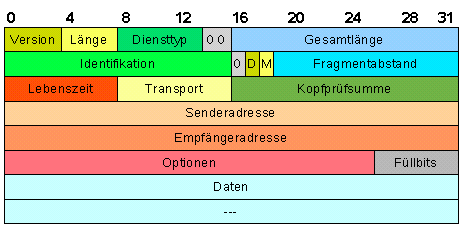
\includegraphics[width=9cm]{img/Datagramms.png}
	\caption{Aufbau eines Datagramms}
	\footnotesize\sffamily\textbf{Quelle:} \url{http://einstein.informatik.uni-oldenburg.de/rechnernetze/diagramm.htm} 
	\label{fig:datagramms}
  \end{center}   
\end{figure}

TCP ist eines der wichtigstens Protokolle der Transportschicht im TCP/IP-Referenzmodell und ist ein zuverlässiges, verbindungsorientiertes und paketvermittelndes Transportprotokoll, welches das Ziel hat, Datenverluste bei der Datenübertragung zu unterbinden, größere Datenmenge in kleinere Pakete zu zerlegen und die empfangene Datenpakete über Ports an den korrekten Anwendungen weiterzuleiten. Da sich TCP ein verbindungsorientiertes Protokoll handelt, definiert das TCP-Protokoll eine Ende-zu-Ende-Verbindung zwischen den Kommunikationspartnern im Netzwerk. (vgl. \cite{o.V.2019})
\\

Das TCP-Protokoll verwendet dabei das Verfahren namens \textit{Positive Acknowledgement (ACK) with ReTransmission\footnote{auf deutsch: positive Bestätigung mit erneuter Übertragung}}, um die Zuverlässigkeit der Datenübertragung sicherzustellen. Dies hat zu bedeuten, dass der Empfänger nach dem Erhalt der Daten dem Sender mit einer positiven Nachricht quittiert wird. Mit einer positiven Nachricht weiß der Sender, dass das Paket den Empfänger erreicht hat. Sollte von seitens der Empfänger keine positive Nachricht kommt, wird das Senden solange wiederholt, bis eine positive Antwort beim Sender eingegangen ist (\textbf {Abbildung \ref{fig:acknowledgement}}). (vgl. \cite{Hol2001})

\begin{figure}[H]
  \begin{center}
    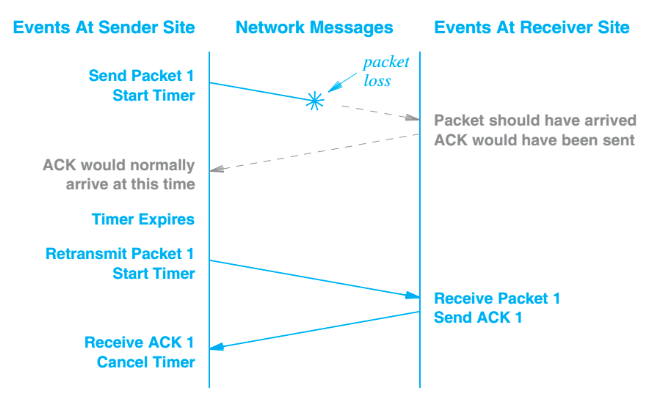
\includegraphics[width=9cm]{img/Acknowledgement.png}
	\caption{Zeitüberschreitung und erneute Übertragung bei Verlust eines Pakets}
	\footnotesize\sffamily\textbf{Quelle:} \url{http://lemoncisco.blogspot.com/2014/06/internetworking-with-tcpip-notes_25.html} 
	\label{fig:acknowledgement}
  \end{center}   
\end{figure}

Die folgende Abbildung (\textbf {Abbildung \ref{fig:tcp}}) zeigt die wichtigsten Protokolle im TCP/IP-Referenzmodell. Über der TCP- und IP-Schicht im TCP/IP-Referenzmodell befindet sich die Anwendungsschicht. Diese Schicht beinhaltet alle Protokolle auf Anwendungsebene, die auf TCP oder UDP aufsetzen. Die Anwendungsschicht stellt den Anwendungsprogrammen Dienste zur Verfügung. Das bekannteste Protokoll auf der Anwendungsschicht ist wohl das Hypertext Transfer Protocol (HTTP), welches den Zugriff auf die Webseiten ermöglicht.

\begin{figure}[H]
  \begin{center}
    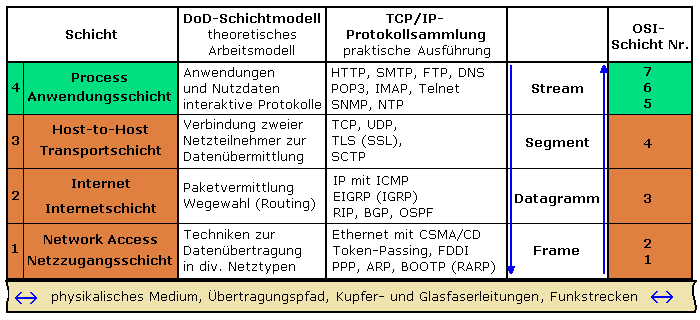
\includegraphics[scale=0.5]{img/tcp.png}
	\caption{Die wichtigsten Protokolle im TCP/IP-Referenzmodell}
	\footnotesize\sffamily\textbf{Quelle:} \url{https://www.elektroniktutor.de/internet/tcpip.html} 
	\label{fig:tcp}
  \end{center}   
\end{figure}

\newpage
\subsection{HTTP}
\label{sec:http}
Das Hypertext Transfer Protocol (HTTP) ist ein zustandsloses und unidirektionales Datenübertragungsprotokoll in einem Netzwerk. Es wird hauptsächlich eingesetzt, um die Dateien vom Server anzufordern und sie in den Browser zu laden und darzustellen. Bei HTTP handelt es sich um eine unverschlüsselte Kommunikation. Dies hat zur Folge, dass alle Informationen im Klartext gesendet werden. Für die verschlüsselte Verbindung bietet sich das sichere HyperText-Übertragungsprotokoll HTTPS\footnote{Hypertext Transfer Protocol Secure} an. HTTP arbeitet nach dem Client-Server-Modell (\textbf {Abbildung \ref{fig:client-server-modell}}). 

\begin{figure}[H]
  \begin{center}
    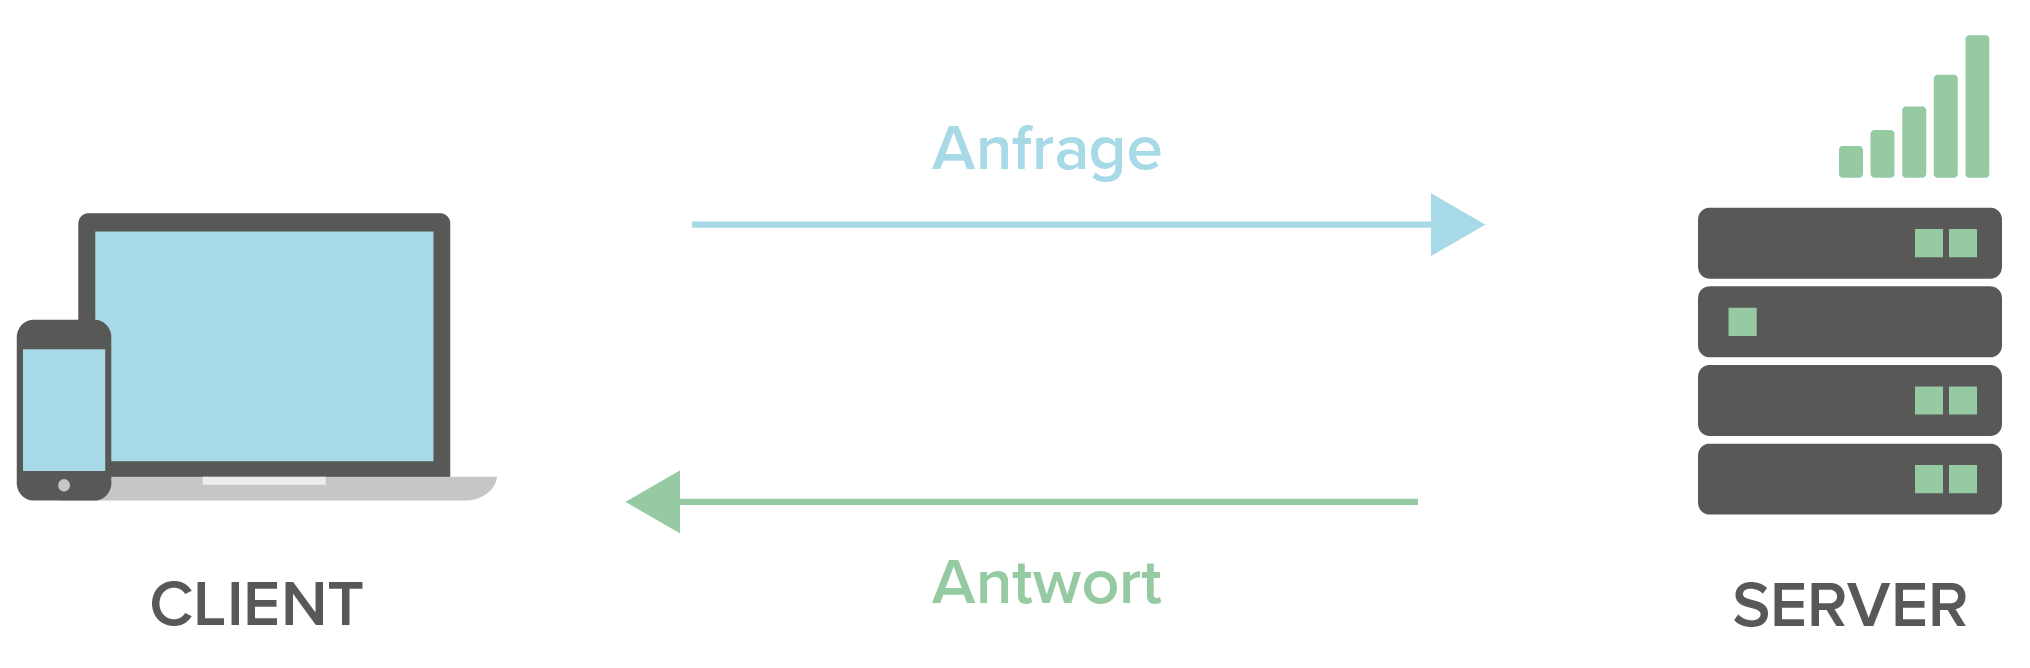
\includegraphics[scale=0.4]{img/client-server-modell.png}
	\caption{Das Client-Server-Modell}
	\footnotesize\sffamily\textbf{Quelle:} \url{https://www.placetel.de/ratgeber/client} 
	\label{fig:client-server-modell}
  \end{center}   
\end{figure}

Der Client (Webbrowser) sendet eine HTTP-Anfrage an den Port 80 des Servers (HTTP-Server). Dieser erledigt die Anfrage vom Client und schickt ihm eine Antwort zurück. Diese Kommunikation verläuft im Textformat. Die Anfrage- sowie die Antwortnachrichten bestehen aus einem Header und Daten. Der Header beinhaltet Steuerinformationen. Der Datenteil enthält den eigentlichen Inhalt der Seite. Nach Abarbeitung der Anfrage wird die Verbindung zwischen Client und Server abgeschlossen. Der Server steht also für die Bearbeitung von neuen Anfragen zur Verfügung. Um dem Server mitzuteilen, was er genau dem Client schicken soll, adressiert der Client bei der Anfrage eine Datei, die sich auf dem Server befindet muss. Dazu verwendet der Client eine URL\footnote{Uniform Resource Locator}. Ist diese Datei vom Client nicht vorhanden, antwortet der Server mit der Fehlermeldung (Error 404) zurück. Für eine zuverlässige Kommunikation verwendet HTTP das verbindungsorientierte Transportprotokoll TCP. (vgl. \cite{Lub2018})

\newpage
Eine URL ist wie folgt aufgebaut\footnote{vgl. \url{https://webdesigneinfuehrung.wordpress.com/tag-8/wie-ist-eine-url-aufgebaut/}}:

\begin{figure}[H]
  \begin{center}
    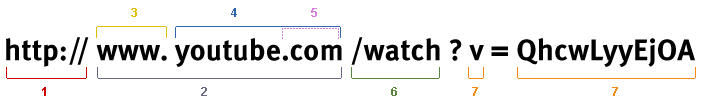
\includegraphics[scale=0.5]{img/url-aufbau.jpg}
	\caption{Aufbau einer URL}
	\footnotesize\sffamily\textbf{Quelle:} \url{https://webdesigneinfuehrung.files.wordpress.com/2013/10/url-aufbau.jpg} 
	\label{fig:url-aufbau}
  \end{center}   
\end{figure}

\begin{enumerate}
\item Das verwendete Protokoll (HTTP). Andere Protokolle könnten ebenfalls verwendet werden, wie HTTPS, FTP.
\item Es handelt sich um der Host oder Hostnamen.
\item Die Subdomain: www (World Wide Web).
\item Die Domain oder der Domainname. Dieser Name ist einmalig wie eine Postanschrift.
\item beschreibt die Top-Level-Domain und bezieht sich auf das Ursprungsland der Webseite.
\item Der Pfad. Dieser verweist auf eine bestimmte Ressource (Datei, Verzeichnis) auf dem Server.
\item Parameter und Wert: v (Parameter), QhcwLyyEjOA (Wert).\\
Nach dem Pfad folgt in dem Beispiel ein URL-Parameter. Er wird durch ein Fragezeichen getrennt.
\end{enumerate}

\subsection{Ablauf einer HTTP-Verbindung}
\label{sec:ablauf einer http-verbindung}
Der Ablauf einer HTTP-Verbindung wird mit dem Beispiel eines Aufrufes einer Webseite im Webbrowser dargestellt. Das Aufrufen einer Webseite im Browser erfolgt hauptsächlich in vier Schritten:

\begin{figure}[H]
  \begin{center}
    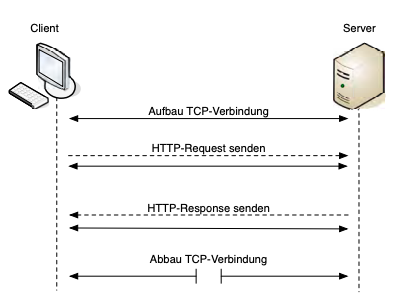
\includegraphics[scale=0.5]{img/http-request-response}
	\caption{Klassisches HTTP Request-Response-Paradigma nach \cite{Wöhr2004}}
	\label{fig:http-request-response}
  \end{center}   
\end{figure}

\newpage
\begin{enumerate}
\item Der Client baut eine TCP-Verbindung zum Server auf.
\item Der Client, in diesem Fall der Benutzer gibt z.B. eine Adresse (URL) in das Adressfeld seines Webbrowsers ein. Diese Adresse wird als HTTP-Request an der Server gesendet.
\item Der Server bearbeitet die Anfrage von dem Benutzer (Client) und antwortet ihm mit einer HTTP-Response zurück.
\item Nach dem Response baut der Server die Verbindung wieder ab.
\end{enumerate}

\subsection{AJAX}
\label{sec:ajax}
AJAX\footnote{Asynchronous JavaScript and XML} ermöglicht, dass die Daten zwischen Browser und Server im Hintergrund austauschen können, ohne die Seite komplett neu zu laden. Man spricht von einer asynchrone Datenübertragung zwischen Client und Server.
\\

Dabei ist das XMLHttpRequest\footnote{kurz: XHR}-Objekt in JavaScript für die Durchführung dieser asynchrone Datenübertragung zwischen Client und Server verantwortlich. XHR ist eine Schnittstelle zwischen JavaScript und Daten auf dem Server. Das XMLHttpRequest sendet eine HTTP-Anfrage an einen Webserver. Die Rückgabe vom Server kann ein JavaScript direkt per DOM\footnote{Document Object Modal} und CSS\footnote{Cascading Style Sheets} in das Dokument ergänzen oder verändert, ohne die Seite neu laden zu müssen. Die statische Inhalte bleiben erhalten, während nur veränderliche Information ergänzt werden. Das spart vor allem Zeit, reduziert den Trafficverbrauch und ermöglicht Nutzer interaktiv mit dem Server zu kommunizieren.
\\

Nach \cite{o.V.2017} unterstützt XHR neben XML-Dokumente auch alle Textformate und kann eine Anfrage ebenfalls über HTTPS übermitteln.
Ein typisches Beispiel für die AJAX-Anwendung ist die Autovervollständigung von Google. Sobald der Nutzer die Daten im Suchfeld auf der Google Webseite eingibt, wird dabei automatisch die passende Vorschläge geliefert. 

\begin{figure}[H]
  \begin{center}
    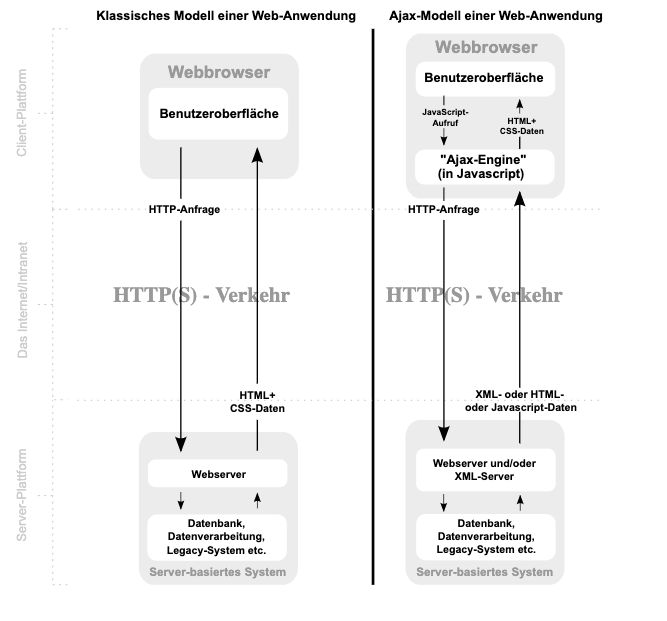
\includegraphics[scale=0.4]{img/ajax-modell}
	\caption{synchrone und asynchrone Kommunikation}
	\footnotesize\sffamily\textbf{Quelle:} By I, DanielSHaischt, CC BY-SA 3.0, https://commons.wikimedia.org/w/index.php?curid=2223689 
	\label{fig:ajax-modell}
  \end{center}   
\end{figure}

\subsection{Echtzeit}
\label{sec:echtzeit}

\chapter{Analyse}
\label{sec:analyse}
Dieses Kapitel der Arbeit betrachtet zunächst den gegenwärtigen Stand der Technik hinsichtlich bereits vorhandenen Tools. Ihre Stärken und Schwächen werden ebenfalls aufgezeigt. Danach geht es um die Anforderungsanalyse der Webanwendung. Dazu wird eine allgemeine Struktur festgelegt, wie die Arbeit systematisch aufgebaut sein soll. Anschließend wird der aktuelle Zustand (Ist-Analyse) des Projektes ermittelt und anhand dieser Ist-Analyse erfolgen die funktionalen und nicht-funktionalen Anforderungen an die zu entwickelnde Webanwendung.

\section{Stand der Technik}
\label{sec:stand der technik}
Bei der Suche nach öffentlich zugänglichen Tools für die Durchführung von Workshops wurden folgenden Ergebnisse gefunden:

\subsection{IdeaBoardz}
\label{sec:ideaBoardz}
IdeaBoardz\footnote{vgl. \url{https://ideaboardz.com/}} ist eine freie webbasierte Anwendung zum Brainstorming, Erstellen einer ToDo-Liste oder zur Retrospektive im agilen Projektmanagement. Mit diesem Tool ist eine Zusammenarbeit möglich. Die beteiligten Personen können entweder zeitgleich oder zu verschiedenen Zeiten ortsunabhängig auf das gemeinsame Dokument zugreifen und bearbeiten. In Echtzeit zusammenarbeiten, ist bei IdeaBoardz nicht realisierbar. Das hat zur Folge, dass bei der Veränderung des Zustands keine sofortige Aktualisierung der Benutzeroberfläche erfolgt. IdeaBoardz wird unter anderem bei Brainstorming-Methode wie die 6-Hüte-Methode\footnote{engl. Six Thinking Hats} von De Bono und auch für die Ideenbewertung bekannte SWOT\footnote{steht für Strengths-Weaknesses-Opportunities-Threats-Analyse}-Analyse angewendet. Die Registrierung ist optional, so dass der Nutzer auch IdeaBoardz verwenden kann, ohne sich anzumelden.

\begin{figure}[H]
  \begin{center}
    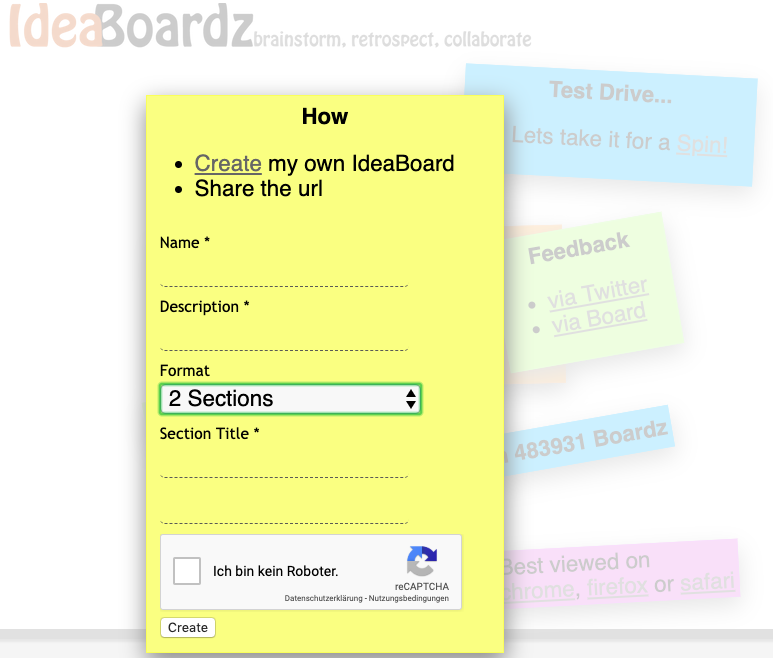
\includegraphics[scale=0.3]{img/ideaBoardz1}
	\caption{Erstellen eines eigenen IdeaBoards} 
	\label{fig:erstellen des eigenen ideaboards}
  \end{center}   
\end{figure}

Die \textbf{Abbildung \ref{fig:erstellen des eigenen ideaboards}} zeigt, wie ein IdeaBoard zu erstellen ist. Neben dem Namen des Boards werden das Thema (Description) und Formate (Format) benötigt. Es können bis zu 10 Sektionen gewählt werden und es stehen noch weitere Formate zur Verfügung, wie Pro und Contra, ToDo-Liste, Six Thinking Hats und vieles mehr. Anschließend wird ein Titel für jegliche Sektionen eingegeben.

\begin{figure}[H]
  \begin{center}
    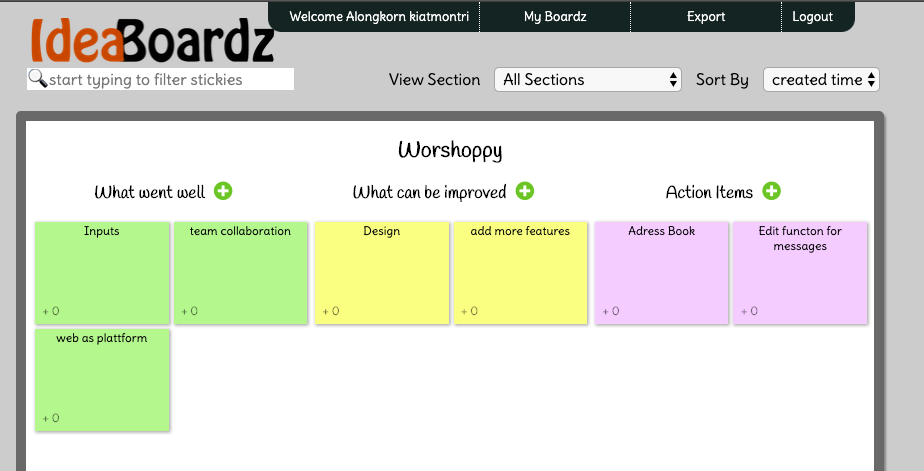
\includegraphics[scale=0.35]{img/ideaBoardz2}
	\caption{Darstellung von Sektionen} 
	\label{fig:darstellung von sektionen}
  \end{center}   
\end{figure}

Wie in \textbf{Abbildung \ref{fig:darstellung von sektionen}} zu sehen ist, sind die Eingaben in Sektionen strukturiert und farbig sortiert. Das Thema steht in der Mitte. Jede Sektion hat einen Titel und einen Plus-Button. Mit diesem Button können zu jeder Sektion neue Eingaben hinzugefügt werden. Die Eingaben werden als Karteikarten bzw. Notizzetteln visualisiert. Der weiße Hintergrund kann wie ein Whiteboard oder eine Pinnwand gesehen werden. Die Eingaben können auch von beteiligten Personen abgestimmt werden. Es ist auch möglich, die Daten nach Datum oder Abstimmung sortieren zu lassen.\bigskip

Als weiteres Feature lassen sich die Sektionen einzeln darstellen (\textbf{Abbildung \ref{fig:darstellung einer der sektionen}}). Die Suche nach dem Eingabeinhalt und das Exportieren der Ergebnisse sowohl in eine PDF-Datei als auch in ein Excel-Dokument werden ebenfalls bei dieser Webanwendung angeboten. Die Daten können sowohl innerhalb als auch außerhalb der Sektion zusammengeführt (Merge) werden. Ebenso lassen sich die Daten aus einer Sektion anderer Daten per Drag \& Drop zuordnen, wie in \textbf{Abbildung \ref{fig:zusammenführen und zuordnen von daten}} zu sehen ist. Mit dem Teilen von URL kann das jeweilige IdeaBoardz für die Zusammenarbeit freigegeben werden.

\begin{figure}[H]
  \begin{center}
    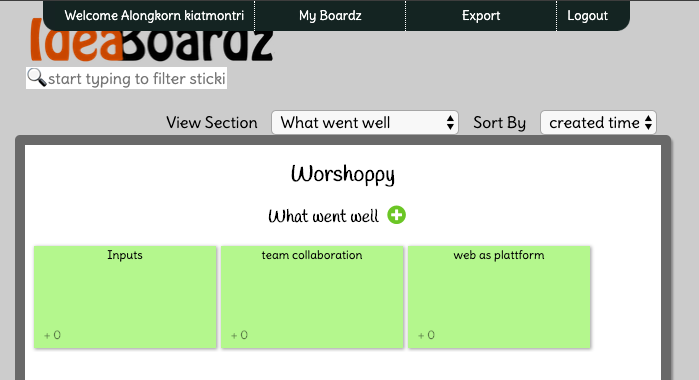
\includegraphics[scale=0.4]{img/ideaBoardz3}
	\caption{Darstellung einer der Sektionen} 
	\label{fig:darstellung einer der sektionen}
  \end{center}   
\end{figure}

\begin{figure}[H]
  \begin{center}
    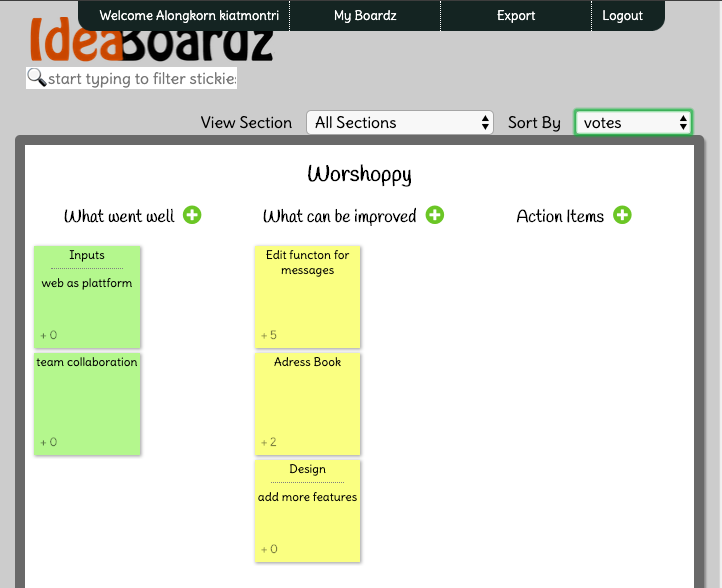
\includegraphics[scale=0.35]{img/ideaBoardz4}
	\caption{Zusammenführen und Zuordnen von Daten} 
	\label{fig:zusammenführen und zuordnen von daten}
  \end{center}   
\end{figure}

\newpage
Einige der oben dargestellten Features können für das Workshoppy-Projekt übernommen werden. Zu nennen sind:

\begin{itemize}
\item Die Eingabe wie ein Notizzettel oder Karteikarten visualisieren.
\item Die Ergebnisse als PDF-Datei exportieren.
\item Eingaben in Sektion darstellen.
\item Zuordnung von Daten (per Drag \& Drop).
\end{itemize}

Mit welchen Webtechnologien IdeaBoardz entwickelt wurde, lässt sich anhand der Informationen auf der Webseite nicht erkennen. Man kann aber davon ausgehen, dass es sich bei IdeaBoardz um eine webbasierte Anwendung mit reichlich Interaktionen auf der Benutzeroberfläche handelt, d.h. es ist über einen Webbrowser nutzbar und der Nutzer muss nichts installieren. Dementsprechend gehört IdeaBoardz zu einer Thin Client-Anwendung und zählt auch zu Rich Internet Applications sowie Web 2.0-Anwendung. (\textbf{siehe Kapitel \ref{sec:grundlagen}}).

\subsection{Miro-RealtimeBoard}
\label{sec:miro-realtimeBoard}
Miro\footnote{vgl. \url{https://miro.com/}} ist eine dynamische Webanwendung und handelt es sich um ein kollaborativer Online-Whiteboard in Echtzeit. Um das Online-Whiteboard nutzen zu können, wird ein Account benötigt. Dafür muss man sich bei Miro registrieren. Miro bietet die kostenlose Version an, sie ist für bis zu drei Teammitglieder und drei Boards geeignet.\bigskip

Begonnen wird mit einer leere Seite oder man verwendet eine von Miro bereitgestellten Vorlage. Zur Vorlage gehören unter anderem MindMap, Flowchart, Brainwriting und Concept Map. Einfügen neuer Dateien, Bilder und Dokumenten aus Google Drive oder vom Rechner ist auch möglich, um Informationen auszutauschen. Der Nutzer kann virtuelle Notizen erstellen. Die Notizen können sich nach Farbe unterscheiden und per Drag \& Drop über das komplette Board verschieben. Mit Hilfe von Share-Button vereinfacht Miro die Teilen-Funktion über eine URL oder einen Gmail-Account das ortsunabhängige und kollaborative Arbeiten in Echtzeit. Somit können die beteiligten Person beispielsweise während des Brainstormings auf die Ideen der anderen eingehen und kommentieren. Außerdem können die Benutzer das Whiteboard in eine Präsentation umwandeln oder in eine PDF-Datei exportieren.\bigskip

Miro ist ebenfalls gut geeignet zur Umsetzung eines klassischen Brainstormings (\textbf{Abbildung \ref{fig:miro board}}). Die Ideen werden in Form von Notizen erstellt. Zusammenfassend können die Notizen nach Farben kategorisiert werden.  

\begin{figure}[H]
  \begin{center}
    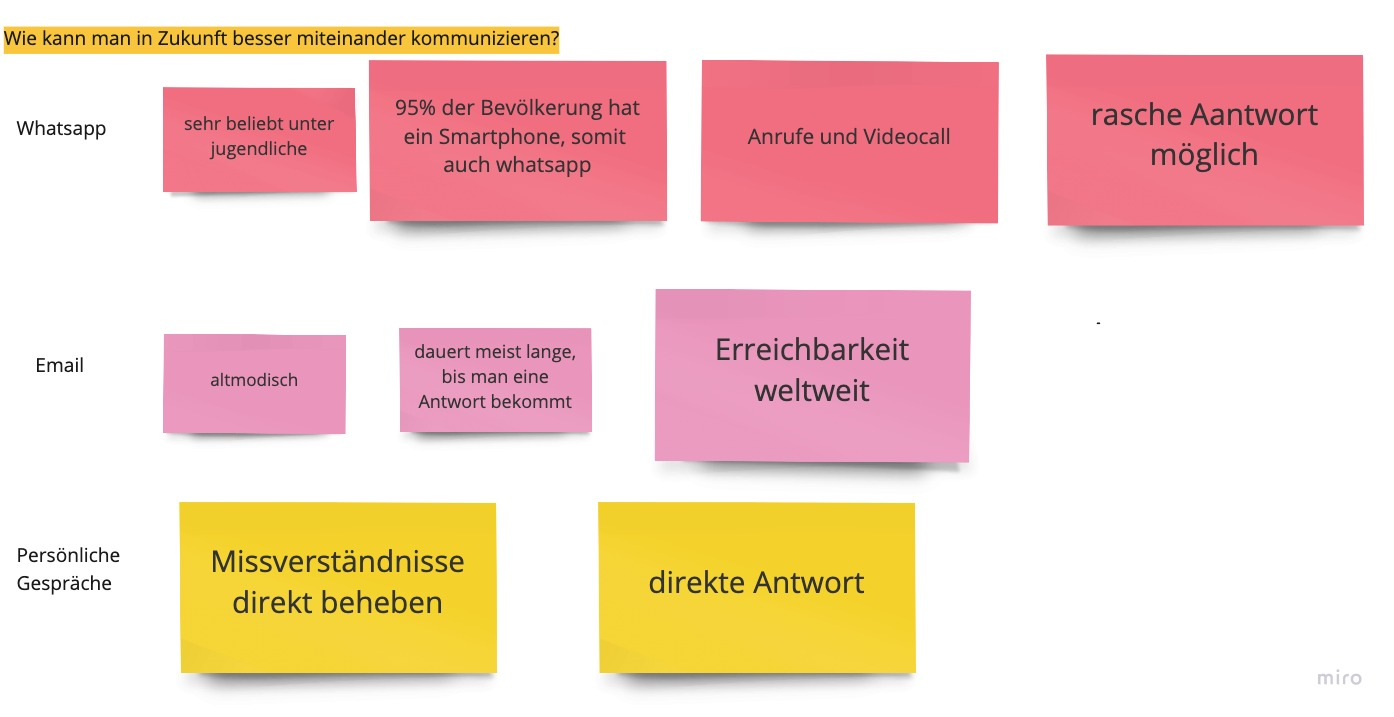
\includegraphics[scale=0.25]{img/miro1}
	\caption{Realisieren eines Brainstormings mit Hilfe von Miro} 
	\label{fig:miro board}
  \end{center}   
\end{figure}

Folgende Erkenntnisse wurden bei der Analyse von Miro gefunden und werden für das Workshoppy-Projekt übernommen: 
\begin{itemize}
\item AJAX-Anwendung
\item Thin Client-Anwendung
\item Web 2.0-Anwendung
\item Rich Internet Applications
\end{itemize}

\subsection{MindMap}
\label{sec:mindmap}
MindMap\footnote{wird häufig auch Mindmapping genannt und versteht sich als Gedankenlandkarte} zählt auch zu den Favoriten unter den Kreativitätstechniken und wird häufig in vielen Workshops als Methode zur Ideenfindung und -strukturierung eingesetzt. Man kann sie beispielsweise auch für Brainstorming, Projektplanung oder Ideensammlung verwenden.\bigskip

Bei einer Mindmap werden Begriffe und deren zugehörigen Beziehungen über eine grafische Darstellung dargestellt. Das Hauptthema oder das Schlüsselwort befindet sich als Knoten kreisförmig in der Mitte. Um das Thema herum wird alles in Form von Hauptästen notiert. Man schreibt auf jeden Hauptast ein Schlüsselwort auf. Verbunden werden sie zum Hauptthema mit Linien. Die Hauptäste bilden die ersten Gedankengänge. Von jedem Hauptast zweigen weitere Nebenäste mit Begriffen ab (\textbf{Abbildung \ref{fig:mindmap}}). 

\begin{figure}[H]
  \begin{center}
    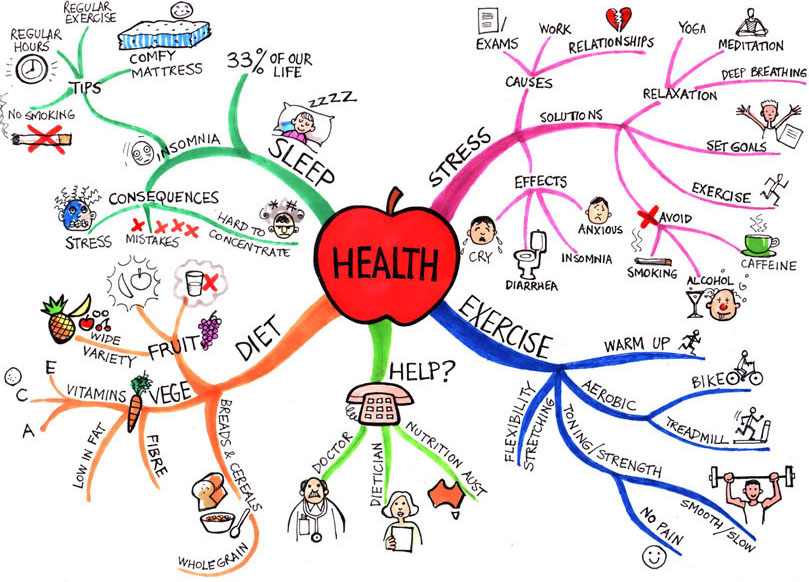
\includegraphics[scale=1.8]{img/health-mindmap}
	\caption{Health mindmap} 
	\footnotesize\sffamily\textbf{Quelle:} Learning Fundamentals: Student Study Techniques by Jane Genovese, Figure 4: Health
mindmap. Online im Internet: URL: \url{https://learningfundamentals.com.au/resources/}  
	\label{fig:mindmap}
  \end{center}   
\end{figure}

Es existieren heutzutage bereits mehrere webbasierte Mindmapping-Tools sowohl kostenlos als auch kostenpflichtig auf dem Markt. Einer von diesen ist, wie bereits im vorherigen Abschnitt vorgestellt, das \textbf{Miro-RealtimeBoard (siehe Abschnitt \ref{sec:miro-realtimeBoard})}, mit dem man Ideen visualisieren und in Echtzeit zusammenarbeiten kann. Die Übersicht zu den anderen Mindmapping-Tools kann auf dieser Webseite\footnote{\url{https://t3n.de/news/mind-mapping-online-tools-568258/}} verfolgt werden.

Neben diesen beiden dargestellten Tools, \textbf{IdeaBoardz} und \textbf{Miro}, gibt es keine weiteren nennenswerte Anwendungen. Zwar gibt es noch zahlreiche Brainstorming-Tools, die in diesem Artikel\footnote{\url{https://tallyfy.com/brainstorming-tools/}} aufgelistet sind. Jedoch sind sie meisten visuell gleich und unterscheiden sich im funktionalen Bereich wenig. Von daher geben sie keine Anreize für diese Arbeit. 

\newpage
\section{Erkennbare Stärken und Schwächen der Konkurrenz-Tools}
\label{sec:erkennbare stärken und schwächen der konkurrenzTools}
\subsection{IdeaBoardz:}
\label{sec:ideaBoardz stärken und schwächen}

\begin{itemize}
\item \textbf{Stärken:}
\begin{itemize}
\item \textbf{Zusammenfügen von Daten per Drag \& Drop:}\\
Die Daten können sowohl innerhalb als auch außerhalb einer Sektion per Drag \& Drop zusammengeführt werden.
\item \textbf{Vote-Funktion:}\\
Den Benutzern wird eine Schaltfläche geboten, mit der sie die Möglichkeit erhalten, Ihr Gefallen für Inhalte von anderen Usern oder von sich selbst auszudrücken. Vergleichbar wie Like-Button\footnote{Gefällt-mir Knopf} auf der Social Media Plattformen.
\item \textbf{Exportieren:}\\
Die Ergebnisse können sowohl als PDF- oder auch als Excel-Datei gespeichert werden.
\item \textbf{Benutzerfreundlichkeit:}\\
Die Webanwendung ist übersichtlich dargestellt, hat eine klare Strukturierung. Sie bietet außerdem eine einfache und verständliche Navigation, hat keinen unnötigen Ballast, wie z.B. Bilder, lange Texte. Sie beinhaltet außerdem kontrastreiche Farben. Die Benutzer erreichen das Ziel mit wenig Aufwand (Klick, Zeit).
\item \textbf{Keine Schulungsaufwand:}\\
Die Webanwendung ist sehr verständlich und leicht zu bedienen. Der Benutzer kommt ohne Schulung gut ans sein Ziel.
\item \textbf{Ohne Registrierung und nicht kostenpflichtig:}\\
IdeaBoardz ist eine kostenlose Webanwendung. Für die Anwendung ist keine Registrierung nötig.
\item \textbf{Responsive Webdesign:}\\
Das Layout der Website ist flexibel gestaltet, dass dieses auf dem Tablet und Smartphone eine gleichbleibende Benutzerfreundlichkeit bietet. 
Der Inhalt der Website wird auf dem mobilen Geräte einheitlich wie auf dem Laptop oder Desktop-Computer dargestellt.
\end{itemize}
\end{itemize}

\begin{itemize}
\item \textbf{Schwächen:}
\begin{itemize}
\item \textbf{Keine Möglichkeit in Echtzeit zusammenzuarbeiten:}\\
Eine der größten Nachteile von dieser Webanwendung ist, dass sie die Daten nicht in Echtzeit liefern kann.  Die Whiteboards können nicht in Echtzeit aktualisiert werden, somit verlaufen die Brainstorming-Sitzungen mit etwas Verzögerung.
\item \textbf{Keine Möglichkeit Thema oder Titel zu editieren: }\\
Das behandelte Thema und die Titel der Sektionen können nach dem Erstellen nicht mehr geändert werden.
\item \textbf{Löschen eines erstellten IdeaBoards und von Sektionen nicht möglich:}\\
Sektionen und das erstellte IdeaBoard können nicht gelöscht werden.
\item \textbf{Daten können nur einmal zusammengeführt werden:}\\
Beim ersten Zusammenführen sind die Daten fest geordnet, d.h. es ist unmöglich, sie einzeln wieder zu trennen oder mit anderen Daten zusammenzuführen. 
\end{itemize}
\end{itemize}

\subsection{Miro-RealtimeBoard:}
\label{sec:stärken und schwächen von miro}
\begin{itemize}
\item \textbf{Stärken:}
\begin{itemize}
\item \textbf{Benutzerfreundlichkeit:}\\
Die Webanwendung hat eine klare Übersicht sowie ein modernes Layout. Sie hat eine klare Strukturierung und bietet eine einfache und verständliche Navigation. Die Werkzeuge sind gut erkennbar, gut strukturiert und verständlich. Die Benutzer erreichen Ihr Ziel mit wenig Aufwand.
\item \textbf{Keine Schulungsaufwand:}\\
Die Webanwendung ist sehr verständlich und leicht zu bedienen. Der Benutzer kommt ohne große Bemühungen gut ans sein Ziel.
\item \textbf{Exportieren:}\\
Miro stellt dem Benutzer die Möglichkeit, die Ergebnisse in verschiedene Formate zu exportieren. Die Ergebnisse können sowohl als PDF- oder auch als CSV-Datei sowie als JPEG-Format gespeichert werden.
\item \textbf{Zusammenarbeit in Echtzeit:}\\
Mit Hilfe von Share-Button vereinfacht Miro die Teilen-Funktion über einen URL oder ein Gmail-Account das ortsunabhängigen und kollaborativen Arbeiten der Teammitglieder in Echtzeit.
\item \textbf{Präsentationsmodus:}\\
Die Ergebnisse können in einem Präsentationsmodus verwandeln werden.
\item \textbf{Chatfunktion:}\\
Die Teammitglieder können sich mittels einem eingebauten Chat Nachrichten untereinander austauschen.
\item \textbf{Hochladen von Dateien:}\\
Fügen neue Dateien, Bilder und Dokumente aus Google Drive oder vom Rechner ist auch möglich.
\item \textbf{Kommentar in Echtzeit hinzufügen:}\\
Durch der eingebauten Kommentarfunktion ist es möglich, das Feedback der Mitglieder in Echtzeit zu erhalten und die Qualität der Inhalte zu verbessern. 
\item \textbf{Verschiedene Vorlage:}\\
Der Benutzer hat die Möglichkeit, verschiedene Vorlagen, wie Mindmapping, User Story-Map, Flowchart, Concept-Map, Brainwriting sowie Wireframing zu verwenden.
\item \textbf{Responsive Webdesign:}\\
Das Layout der Website ist flexibel gestaltet. Das einheitliche Anzeigen von Inhalten wird auf allen Endgeräte (Laptop, Ipad, Smartphone) gewährleistet. Somit kann der Inhalt gänzlich und schnell vom Benutzer aufgenommen werden.
\end{itemize}
\end{itemize}

\begin{itemize}
\item \textbf{Schwächen:}
\begin{itemize}
\item \textbf{Registrierung notwendig:}\\
Bei dieser Webanwendung ist ein Account notwendig. Der Benutzer muss sich bei Miro registrieren.
\item \textbf{Begrenzte Funktion bei der kostenlosen Version:}\\
Die kostenlose Version ist auf bis zu drei Mitglieder und drei Boards erlaubt. Die Funktionen ist bei der kostenlosen Version begrenzt. Ein Upgrade auf 40 \$ pro Monat bringt zwei weitere Teammitglieder, unbegrenzte Boards sowie Funktionen.
\end{itemize}
\end{itemize}

Die \textbf{Tabelle \ref{tab:konkurrenten vergleich}} stellt zusammenfassend die Funktionsüberblick der beiden Konkurrenz-Tools vor.
\newcolumntype{C}[1]{>{\centering\arraybackslash}m{#1}}
\begin{table}[H]
	\centering
	\begin{tabular}{|c|c|C{3cm}|}
	\hline
	\textbf{Funktion} & \textbf{IdeaBoardz} & \textbf{Miro}\\
	\hline
	In Echtzeit zusammenarbeiten & Nein & Ja\\
	\hline
	Präsentationsmodus & Nein & Ja\\
	\hline
	Hochladen von Dateien & Nein & Ja\\
	\hline
	Vote-Funktion & Ja & Nein\\
	\hline
	Benutzerfreundlichkeit & Ja & Ja\\
	\hline
	kostenlos & volle Funktionen & begrenzte Funktionen und Mitglieder\\
	\hline
	Registrierung & Nein & Ja\\
	\hline
	Exportieren in andere Formate, z.B. in PDF-Datei & Ja & Ja\\
	\hline
	Responsive & Ja & Ja\\
	\hline
	Schulungsaufwand & Nein & Nein\\
	\hline
	Verschiedene Vorlagen, z.B. Mind Map & Nein & Ja\\
	\hline
	\end{tabular}
	 \caption{Funktionsüberblick der beiden Konkurrenzen.}
	 \label{tab:konkurrenten vergleich}
\end{table}

\section{Projektstruktur}
\label{sec:projektstruktur}
Im folgenden wird der geplante Projektablauf in Form eines Projektstrukturplans\footnote{Nach Definition der DIN 69901-5:2009 ist der Projektstrukturplan die \textit{\glqq [...] vollständige hierarchische Darstellung aller Elemente (Teilprojekte, Arbeitspakete) der Projektstruktur als Diagramm oder Liste.\grqq{}}} dargestellt:\bigskip

Auf der obersten Ebene steht das Projekt. Eine Ebene darunter die Teilprojekte oder Teilaufgaben, darunter schließlich die Arbeitspakete. Der Projektstrukturplan (\textbf{Abbildung \ref{fig:projektstruktur}}) entspricht dem typischen sequentiellen Vorgehensmodell zur Softwareentwicklung einschließlich der Entwicklung der Webanwendung. 

\begin{figure}[H]
  \begin{center}
    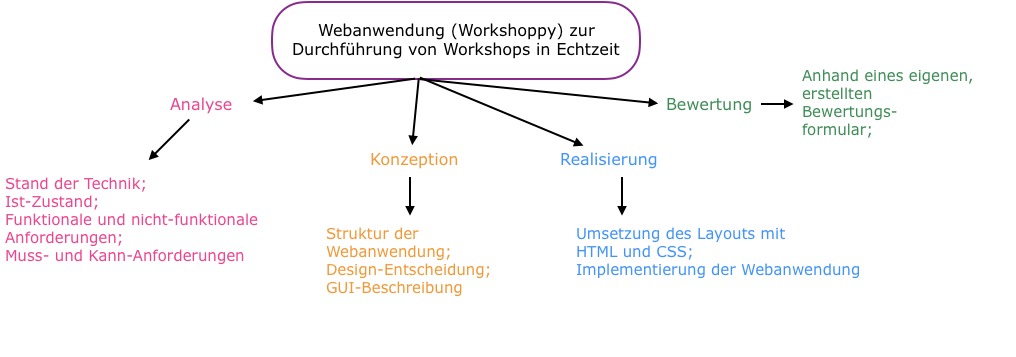
\includegraphics[scale=0.4]{img/projektstruktur}
	\caption{Projektstrukturplan} 
	\footnotesize\sffamily\textbf{Quelle:} eigene Abbildung  
	\label{fig:projektstruktur}
  \end{center}   
\end{figure}

Die Konkurrenz-Tools und eine Analyse von funktionalen, nicht-funktionalen Anforderungen sowie die Muss- und Kann-Anforderungen werden in der ersten Phase untersucht. Durch diese Analyse wird die Struktur und ein passendes Layout der Webanwendung erstellt. Die daraus entstehende Designentscheidung wird technisch in eine Webanwendung umgesetzt und am Ende wird die Webanwendung anhand eines selbst erstellten Bewertungsformulars von den Mitarbeiter im Unternehmen (mindestens 2 Personen) bewertet.

\newpage
\section{Ist-Analyse}
\label{sec:istAnalyse}
Bei der Projektvorstellung wurde in der Firma zunächst über den Zustand der aktuellen Lösungen für die Durchführung von Workshops gesprochen.\bigskip

Wie der Abschnitt \textbf{Stand der Technik (Abschnitt \ref{sec:stand der technik})} aufgezeigt hat, existieren bereits zahlreiche webbasierte Tools für die Durchführung von Workshops.\bigskip

Nach der Betrachtung der aktuellen Lösungen fällt das Fazit des Unternehmens folgendermaßen aus: Die vorhandenen Tools reichen noch nicht aus, um Workshops effektiv durchzuführen. Während \textbf{IdeaBoardz \ref{sec:ideaBoardz}} keine Zusammenarbeit in Echtzeit bieten kann, hat \textbf{Miro \ref{sec:miro-realtimeBoard}} bei der kostenlosen Version eine begrenzte Anzahl an Teammitgliedern, d.h. Workshops mit mehr als drei Teilnehmer muss deshalb die kostenpflichtige Version verwendet werden. Außerdem bereiten die aktuellen Lösungen viel Mühe in puncto Dateneingabe. Besonders auf dem Smartphone-Bildschirm ist die Dateneingabe sehr fummelig und nicht komfortabel. Das Smartphone scheint für eine Arbeit mit der aktuellen Lösungen überfordert zu sein. \bigskip

Als weitere und oft eingesetzte Methode zum Brainstormen in den Workshops ist das Mindmapping. Es ist eine Form, die beim Brainstorming entstehenden Ideen bildlich zu strukturieren. Jedoch hat die Mindmapping-Methode auch ihre Nachteile. Man muss sich zunächst an diese Form der Aufzeichnung gewöhnen. Denn MindMaps sehen auf den ersten Blick unübersichtlich und verschachtelt aus. Diese können sehr schnell ihre Übersichtlichkeit verlieren, wenn verschiedene Schlüsselwörter in Beziehung stehen. Demzufolge ist die Akzeptanz der Nutzer, die mit dieser Methode bzw. dieser Aufzeichnung nicht vertraut sind, eher gering. Es ist außerdem sehr zeitaufwendig, eine Mindmap exakt nach den Regeln zu erstellen. Mindmaps sind eher für den individuellen Gebrauch geeignet, da die verwendeten Schlüsselbegriffe und die Strukturierungen häufig für andere Personen unverständlich sind.\bigskip

Es lässt sich nicht verhindern, dass eine neue Lösung benötigt wird, um das aktuelle Problem zu lösen und vor allem die Durchführung von Workshops effektiver zu gestalten.

\section{Unternehmensanforderungen}
\label{sec:unternehmensanforderungen}
In diesem Abschnitt werden die Unternehmensanforderungen an die zu entwickelnden Lösung besprochen.\bigskip

Die neue Lösung soll eine benutzerfreundliche Webanwendung sein, die intuitiv bedienbar sein soll. Der Moderator übernimmt die Rolle des Administrators und ist hauptverantwortlich für die Steuerung der Webanwendung. Das Brainstorming soll in einer Sitzung (Session) durchgeführt werden. In dieser Sitzung wird versucht, möglichst viele Ideen für ein zuvor klar definiertes Problem zu produzieren. Ein Workshop sollte nicht nur auf eine Sitzung beschränken. Es sollte möglich sein, in einem Workshop mehrere Brainstorming-Sitzungen abwickeln zu können.\bigskip

Die teilnehmenden Personen wiederum sind nur für die inhaltlichen Beiträge zuständig. Die neue Lösung sollte so entwickelt werden, dass die Teilnehmer besonders auf Ihren Mobilgeräten ohne mühevolle Tipperei und ohne großen Aufwand Ihre Ideen abgeben können. Die Ideen sollen dann in Echtzeit für alle sichtbar dargestellt werden, welche nach der Sammlungsphase digital vom Moderator durch ein einfaches zu bedienendes User Interface zusammengefasst werden können/müssen.\bigskip

Die weiteren Hauptkriterien für die neue Lösung sind:
\begin{itemize}
\item Login-Bereich (Moderator)
\item QR-Code zur Teilnahme am Workshop (Teilnehmer)
\item Thin Client-Anwendung
\item Rich Internet Applications
\item Responsive Webdesign 
\item Browserunabhängigkeit
\item Export der Ergebnisse in eine PDF-Datei
\end{itemize}

\section{Anforderungsanalyse}
\label{sec:anforderungsanalyse}
Dieses Kapitel umfasst die grundlegenden Anforderungen dieser Bachelorarbeit. Die Anforderung wird in funktionalen und nicht-funktionalen Anforderungen aufgeteilt.\bigskip

Eine funktionale Anforderung wird nach der Definition aus dem Buch \cite{Balzert2010} die gewünschte Funktionalität des Systems bzw. eines Produkts beschrieben. Die nicht-funktionalen Anforderungen sind Anforderungen, die für die Nutzung des Systems wichtig sind. Außerdem werden Muss- und Kann- Anforderungen formuliert, welche für das Projekt oberste Priorität haben und welche eher zweitrangig sind.

\subsection{Funktionale Anforderungen}
\label{sec:funktionale anforderungen}
Aus den Unternehmensanforderungen \textbf{(Abschnitt \ref{sec:unternehmensanforderungen})} lassen sich folgenden funktionalen Anforderungen ableiten.

\begin{enumerate}
\item \textbf{Der Moderator soll sich über ein Anmeldeformular anmelden können.}\\
Eine dem Moderator bekannte URL führt auf die Willkommensseite der Webanwendung. Dort wird er über ein Anmeldeformular aufgefordert, seinen Benutzernamen und Passwort einzugeben. Das System vergleicht die Eingabe mit der in Datenbank angelegten Nutzerdaten. Gelingt die Anmeldung, wird auf die Hauptseite weitergeleitet. Wenn dem System die Anmeldung nicht bekannt ist, wird eine entsprechende Fehlermeldung angezeigt und die Willkommensseite verbleibt. Für die vorliegende Arbeit werden die Nutzerdaten manuell in einem Datenbanksystem erstellt. Der Registrierungsvorgang wird für die zukünftige Weiterentwicklung im letzten Kapitel festgehalten. 
\item \textbf{Der Moderator soll sich mittels einer Navigationselement abmelden können.}\\ 
Jede moderne Webanwendung bietet dem eingeloggten Nutzer die Möglichkeit, sich ordnungsgemäß auszuloggen. Mit dem Element \glqq Ausloggen\grqq{} in der Navigationsleiste kann sich der Moderator abmelden und er wird zur Willkommensseite weitergeleitet.
\item \textbf{Der Moderator soll neue Workshops erstellen, sie bearbeiten und löschen können.}\\
Der moderierende Person soll die Möglichkeit haben, neue Workshops anzulegen. Die erstellten Workshops werden in eine Liste angezeigt und sollen von dem Moderator bearbeitet und gelöscht werden können. Die Workshops sollten in einer Datenbank gespeichert werden.
\item \textbf{In einem Workshop sollen eine oder mehreren Sitzungen (Sessions) für Ideenfindung und -sammlung erstellt werden können.}\\
Eine Session versteht sich als eine Sitzung, um Lösungen für Problemstellung zu generieren, verschidene Themen aufzuarbeiten oder Entwicklung neuer Geschäftsideen sowie Innovationen zu fördern. Der Moderator soll in einem Workshop eine oder mehreren Sitzungen (Sessions) erstellt werden können. Er sollte die erstellten Sessions auch bearbeitet und gelöscht werden können. Die Sessions sollten ebenso in einer Datenbank gespeichert werden.
\item \textbf{Die teilnehmenden Personen sollen über einen QR-Code oder eine Einladungsmail an dem jeweiligen Workshop mitwirken können.}\\
Zu Beginn des Workshops sollte ein QR\footnote{englisch: Quick Response}-Code mittels Beamer angezeigt werden, sodass die anwesenden Teilnehmer diesen mit ihren Mobilgeräten einscannen und an diesem Workshop mitwirken können. Der Moderator sollte auch die Möglichkeit haben, auch während einer Sitzung den QR-Code einblenden zu können. Die Einladung zur Teilnahme am Workshop sollte ebenfalls auch per Mail gesendet werden können.
\item \textbf{Die Teilnehmer sollen auf ihren Endgeräte Ihre Ideen abgeben können.}\\
Sobald eine Sitzung eines Workshops gestartet ist, sollten auf den Endgeräten der Teilnehmer zunächst ein Eingabefeld für Benutzernamen erscheinen. Dort werden sie aufgefordert, einen Benutzernamen einzugeben. Nach der Eingabe des Benutzernamens soll eine Textarea für die Dateneingabe freigeschaltet werden. Über diese sollen die Teilnehmer Ihre Gedanken und Vorschläge frei äußern können. Außerdem sollte es den Teilnehmern möglich sein, Ihren Benutzernamen zu ändern.
\item \textbf{Die Dateneingabe der Teilnehmer sollen auf dem Beamer in Echtzeit angezeigt werden können.} \\
Die eingegebenen Daten der Teilnehmer sollen in Echtzeit auf der Präsentation-Seite, welche parallel über dem Beamer läuft, präsentiert werden.
\item \textbf{Der Moderator soll die Daten in Kategorien zusammenfassen können.}\\
Die Sammlungsphase ist beendet und der Moderator wird anschließend mit der Gruppe die Ergebnisse auswerten und sortieren. Es soll dem Moderator erlaubt sein, die Ergebnisse direkt auf der Präsentation-Seite per Drag \& Drop in Kategorien zusammenzufassen. Die erstellten Kategorien sollen bearbeitet sowie gelöscht werden können. Sie sollten auch in einer Datenbank gespeichert werden.
\item \textbf{Beim Löschen von Kategorien sollen die darin befindlichen Daten nicht betroffen sein.}\\
Beim Löschen einer nicht leeren Kategorie, sollen die darin befindlichen Daten erhalten bleiben. Es wird nur die Kategorie gelöscht.
\item \textbf{Die Ergebnisse sollen in eine PDF-Datei exportiert und heruntergeladen werden können.}\\
Nach Beendigung des Workshops sollen die Daten digital von allen Sitzungen zusammengefasst und als PDF-Datei heruntergeladen werden können. Der beendete Workshop soll dann in einer separaten Liste archiviert werden.
\end{enumerate}

\subsection{Nicht-funktionale Anforderungen}
\label{sec:nicht-funktionale anforderungen}
Im oberen Unterkapitel wurden die funktionalen Anforderungen aufgelistet. In diesem Kapitel werden die nicht-funktionalen Anforderungen formuliert, welchen zu diesem Projekt gehören sollen.

\begin{itemize}
\item \textbf{Layout, Handhabung und Benutzbarkeit}\\
Gemessen am Funktionsumfang sollte die zu entwickelnde Anwendung ein möglichst strukturiertes, einfaches und bedienerfreundliches Layout besitzen. Beim Entwurf und der Entwicklung der Anwendung sollten deshalb die folgenden Punkte beachtet werden:
\begin{itemize}
\item Die Verwendung der Webanwendung soll für Nutzer intuitiv sein. Der Nutzer soll mit wenigem Aufwand, ohne besondere Schulung und in kurzer Zeit durch die Webanwendung navigieren sowie sie verwenden und die wichtigen Funktionen der Webanwendung ausführen können.
\item Bereitstellung von Hilfeleistung in Form von Hilfetexten und Tooltips zur Förderung der intuitiven Bedienbarkeit.
\item Die Buttons sollen in unterschiedlichen Farben entsprechend der Funktionalität gestaltet werden.
\item Anzeigen von Bestätigungsdialogen beim Löschen von Workshops, Sessions und Kategorien sowie beim Beenden von Workshops.
\item Die Gestaltung der Webanwendung soll einheitlich nach vorgegebenen Designvorlagen vom Unternehmen erfolgen.
\end{itemize}
\item \textbf{Plattformübergreifend}\\
Die Webanwendung soll unabhängig der Plattform funktionieren. Deshalb sollte die Webanwendung nach \textbf{responsive Webdesign} gestaltet werden. Das bedeutet, die Inhalts- und Navigationselemente sowie der strukturelle Aufbau der Webanwendung sollten sich der Bildschirmauflösung aller Endgeräte anpassen. Somit ist es für den Nutzer möglich, diese Anwendung auf verschiedenen Endgeräten zu betreiben.
\item \textbf{Browserunabhängigkeit}\\
Außer der Plattformunabhängigkeit sollte die Anwendung in unterschiedlichen Browsern, wie Firefox oder Chrome genutzt werden können.
\item \textbf{Thin Client-Anwendung}\\
Die Webanwendung soll eine Thin Client-Anwendung sein, dies bedeutet, dass die Anwendung nicht mehr auf jedem Client installiert werden muss, sondern über einen Webbrowser abrufbar und nutzbar ist. Das Updaten von Programmen sowie applikationsspezifische Funktionalitäten werden von Server zur Verfügung gestellt. Da alles über den Webbrowser abläuft, ist eine Thin Client-Anwendung hardware-, sprach- und betriebssystemunabhängig. Für JavaScript- bzw. AJAX-Anwendungen müssen keine weiteren Plug-Ins installiert werden, da die meisten Browser JavaScript unterstützen. 
\item \textbf{Performance}\\
Die eingegeben Daten seitens der Teilnehmer sollten ohne Verzögerung auf der Präsentation-Seite angezeigt werden.
\end{itemize}

\subsection{Muss- und Kann-Anforderungen}
\label{muss- und kann-Anforderungen}
Die funktionalen Anforderungen sowie nicht-funktionalen Anforderungen wurden bereits im Unterkapitel \textbf{\ref{sec:funktionale anforderungen}} und \textbf{\ref{sec:nicht-funktionale anforderungen}} dargestellt. In diesem Kapitel werden die Muss- und Kann-Anforderungen formuliert. Die Muss-Anforderung wird mit Priorität \glqq Hoch\grqq{} gekennzeichnet, für die Kann-Anforderung wird die Priorität auf \glqq Niedrig\grqq{} gesetzt.

\newcolumntype{B}[1]{>{\centering\arraybackslash}m{#1}}
\definecolor{TableHeadGray}{gray}{.8}
\begin{table}[H]
	\centering
	\begin{tabular}{|c|B{10cm}|c|}
	\hline
	\textbf{Merkmal} & \textbf{Anforderung} & \textbf{Priorität}\\
	\hline
	FA & Erstellen, Bearbeiten und Löschen von Workshops & \textbf{Hoch}\\
	\hline
	FA & Auflisten von Workshops & \textbf{Hoch}\\
	\hline
	FA & Archivieren und Anzeigen von beendeten Workshops & \textbf{Hoch}\\
	\hline
	FA & Anmeldeformular für die Moderation & \textbf{Hoch}\\
	\hline
	FA & Der Moderator muss sich ausloggen können & \textbf{Hoch}\\
	\hline
	FA & Erstellen, Bearbeiten und Löschen von Sessions & \textbf{Hoch}\\
	\hline
	FA & QR-Code für die Teilnahme am Workshop & \textbf{Hoch}\\
	\hline
	FA & Die Teilnehmer werden zu Beginn des Workshop aufgefordert, einen Benutzernamen einzugeben & \textbf{Hoch}\\
	\hline
	FA & Benutzernamen ändern & \textbf{Hoch}\\
	\hline
	FA & Dateneingabefunktion & \textbf{Hoch}\\
	\hline
	FA & Dateneingabe in Echtzeit auf der Präsentationsseite darstellen & \textbf{Hoch}\\
	\hline
	FA & Erstellen, Bearbeiten und Löschen von Kategorien & \textbf{Hoch}\\
	\hline
	FA & Beim Löschen von Kategorien sollen die darin befindlichen Daten erhalten bleiben & \textbf{Hoch}\\
	\hline
	FA & Daten in Kategorien zusammenfassen & \textbf{Hoch}\\
	\hline
	FA & Die Ergebnisse sollen in eine PDF-Datei exportiert und heruntergeladen werden können & \textbf{Hoch}\\
	\hline
	NFA & Responsive Webdesign & \textbf{Hoch}\\
	\hline
	NFA & Browserunabhängigkeit & \textbf{Hoch}\\
	\hline
	NFA & Performance & \textbf{Hoch}\\
	\hline
	NFA & Anzeigen von Bestätigungsdialogen beim Löschen von Workshops, Sessions und Kategorien sowie beim Beenden von Workshops & \textbf{Hoch}\\
	\hline
	NFA & Thin Client-Anwendung & \textbf{Hoch}\\
	\hline
	FA & Einladungsmail zur Teilnahme am Workshop & \textbf{Niedrig}\\
	\hline
	NFA & Bereitstellung von Hilfeleistung in Form von Hilfetexten und Tooltips zur Förderung der intuitiven Bedienbarkeit & \textbf{Niedrig}\\
	\hline
	NFA & Die Buttons sollen in unterschiedlichen Farben entsprechend der Funktionalität gestaltet werden & \textbf{Niedrig}\\
	\hline
	NFA & Die Gestaltung der Webanwendung soll einheitlich nach vorgegebenen Designvorlagen vom Unternehmen erfolgen & \textbf{Niedrig}\\
	\hline
	\end{tabular}
	 \caption{Muss- und Kann-Anforderungen}
	 \footnotesize\sffamily FA = Funktionale Anforderung\\
	 NFA = Nicht-funktionale Anforderung 
	 \label{tab:muss- und kann-anforderungen}
\end{table}

\section{Beispielszenario}
\label{beispielszenario}
In diesem Abschnitt wird die zu entwickelnden Webanwendung anhand eines Beispielszenarios näher beschrieben.\bigskip

Man stelle sich folgende Situation vor: Sie führen ein Unternehmen und suchen für ein Problem eine Lösung. Hier sind also die Ideen gefragt. Sie laden alle Abteilungsleiter in den Besprechungsraum ein und führen dazu einen Workshop, um die Lösungsansätze zu erarbeiten. Beim Erarbeiten von Ergebnissen spielt dabei die hierarchische Position im Unternehmen keine Rolle. In einem Workshop ist jeder \glqq gleich\grqq{}.\bigskip

Sie übernehmen die Rolle eines Moderators und erläutern den teilnehmenden Personen das zu behandelnde Problem, die Regeln sowie das Ziel des Workshops. Als Werkzeug für die Durchführung des Workshops steht Ihnen die zu entwickelnden Webanwendung zur Verfügung. Bevor Sie mit dem Workshop beginnt, legen Sie bei der Webanwendung einen Workshop und die dazugehörige Session an.\bigskip

In diese Session findet die Ideenfindungsphase statt. Jeder der im Besprechungsraum anwesenden Teilnehmer scannt den angezeigten QR-Code ein, um an diesem Workshop teilnehmen zu können. Danach kommt jeder dran und gibt auf seinem Endgerät Ideen für die Lösung des Problems ein. Jede eingebrachte Idee wird mittels Beamer in Echtzeit präsentiert.  Die Ideenfindungsphase ist vorüber. Sie als Administrator beendet die Eingabephase auf der Webanwendung. Hier können die anwesenden Teilnehmer keine Ideen mehr eingegeben werden. Sie haben jetzt die Aufgabe, die gesammelten Ideen gemeinsam mit der Gruppe zu analysieren und anschließend zusammenzufassen. Am Ende des Workshops steht Ihnen die Ergebnisse als digitale Dokumentation bereit.




\chapter{Design}
\label{sec:design}
Aus den gesammelten Anforderungen vom \textbf{Kapitel \ref{sec:analyse}} wird es in diesem Kapitel um den Entwurf der Weboberfläche (WebUI) gehen. Die grundlegende Gestaltungsrichtlinie darunter die einheitliche Verwendung von Icons, Farben und Schriftgestaltung werden dabei beschrieben. Außerdem wird der Aufbau der zu entwickelnden Webanwendung mithilfe von Mockups dargestellt.\bigskip

\par
\begingroup
\leftskip=4em % Parameter anpassen
\rightskip\leftskip
\noindent \glqq Gutes Design ist so wenig Design wie möglich
Weniger Design ist mehr, konzentriert es sich doch auf das Wesentliche, statt die Produkte mit Überflüssigem zu befrachten. Zurück zum Puren, zum Einfachen!\grqq{} - Dieter Rams (vgl. 10 Thesen für gutes Design\footnote{\url{https://www.vitsoe.com/de/ueber-vitsoe/gutes-design}})
\par
\endgroup
\bigskip

\section{Gestaltungsrichtlinie}
\label{sec:gestaltungsrichtlinie}
Um der Webanwendung ein einheitliches, strukturiertes und benutzerfreundliches Design zu geben ist es erforderlich, feste Layoutvorgaben zu definieren. Sie sorgt für eine verständliche und intuitiv bedienbare Benutzeroberfläche, sodass eine positive Empfindung der Nutzer bei der Bedienung der Webanwendung hervorgerufen wird und ohne größere Einarbeitungszeit beherrscht werden kann. Diese Vorgabe wird auf alle Seiten der Webanwendung angewendet.

\subsection{Farben}
\label{subsec:farben}
Um die Webanwendung übersichtlich zu halten, wird auf die Verwendung mehrerer Farben verzichtet. Es werden grundsätzlich die Farben grau und weiß verwendet. Die Gestaltung von Buttons und Daten werden wiederum mit bunten Farben gestaltet, damit sie optisch auffallend sind.

\subsection{Schriftgestaltung}
\label{subsec:schriftgestaltung}
Bei der Schriftgestaltung, wie Schriftgröße und Schriftart, ist darauf zu achten, dass sie eine gute Lesbarkeit und ein modernes Aussehen bieten. Deshalb wird eine Schriftart verwendet, bei der es sich um eine serifenlose Schrift handelt.

\subsection{Icons}
\label{subsec:icons}
Die Buttons werden mit Icons gestaltet, um Inhalte schneller zu verstehen und den Nutzen der Funktionen zu verdeutlichen. Hierbei handelt es sich um allgemein übliche und bei mobilen Anwendungen bekannte Icons. Sie sind so gewählt, dass sich der Nutzer bei den grundlegenden Funktionen auf der Webanwendung schnell zurechtfindet. Bei den Icons handelt es sich hierbei um keine Grafiken, sondern um eine sogenannte Icon Fonts, welche über eigenes Stylesheet geladen werden. Die Fonts haben vor allem den Vorteil, dass sie auf jede Bildschirmgröße skaliert werden können. Für diese vorliegende Arbeit werden die Icon Fonts von Font Awesome\footnote{vgl. \url{https://fontawesome.com/}} verwendet.\bigskip

\begin{figure}[H]
  \begin{center}
    
\includegraphics[scale=0.5]{img/icons}
	\caption{Verwendete Icon Fonts} 
	\footnotesize\sffamily\textbf{Quelle:} \url{https://fontawesome.com/icons?d=gallery}  
	\label{fig:icons}
  \end{center}   
\end{figure}

\newpage
\section{Konzeption}
\label{sec:konzeption}
In diesem Abschnitt werden die erstellten Mockups, also die Wireframes der verschiedenen Seiten dargestellt und erläutert. Die definierte Gestaltungsrichtlinie sollte hierbei bei der Konzeption eingehalten werden.

\subsection{Mockup der Willkommensseite}
\label{subsec:mockup der willkommensseite}
Wenn die richtige URL aufgerufen wird, erscheint die Willkommensseite mit der Aufforderung zur Eingabe von Benutzernamen und Passwort \textbf{(Abbildung \ref{fig:mockup für die anmeldung})}. Zur Erinnerung, die Benutzerdaten werden in dieser Arbeit manuell in der Datenbank angelegt. Der Registrierungsvorgang wird in dieser Arbeit nicht vorhanden sein. Dieser wird für die zukünftige Weiterentwicklung festgehalten.\bigskip

Die Formulardaten werden über den Anmelde-Button verschickt, welcher ein Ereignis (Event) auslöst, um den richtigen User zu authentifizieren. Falls der User nicht existiert, wird eine Fehlermeldung auf der Seite ausgegeben \textbf{(Abbildung \ref{fig:mockup für die anmeldungsfehler})}.\bigskip

\begin{figure}[H]
	\centering
  \begin{minipage}[t]{0.45\linewidth}
  	    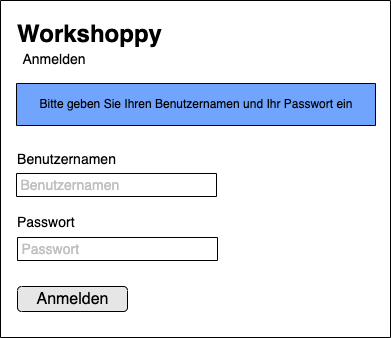
\includegraphics[width=.75\linewidth]{img/willkommenseite1}
		\caption{Mockup für die Anmeldung}
		\label{fig:mockup für die anmeldung}
  \end{minipage}
\hfill
  \begin{minipage}[t]{0.45\linewidth}
    	    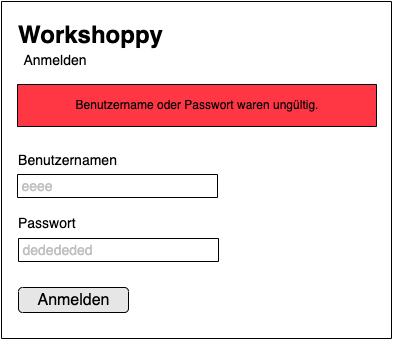
\includegraphics[width=.75\linewidth]{img/willkommenseite2}
		\caption{Mockup für den Anmeldungsfehler}
		\label{fig:mockup für die anmeldungsfehler}
  \end{minipage}
\end{figure}

\newpage
\subsection{Mockup der Hauptseite}
\label{subsec:mockup der hauptseite}
Nach der erfolgreichen Anmeldung wird der Nutzer, der für die Durchführung des Workshops verantwortlich ist, auf die Hauptseite weitergeleitet \textbf{(Abbildung 4.3)}. Auf dieser Seite sind drei grundlegende Bereiche (Nr.1, Nr.2 und Nr.3) zu sehen:\bigskip

\begin{figure}[H]
  \begin{center}
    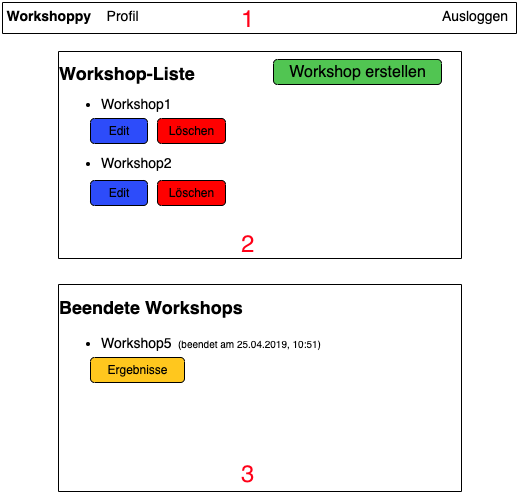
\includegraphics[scale=0.45]{img/hauptseite}
	\caption{Mockup der Hauptseite}  
	\label{fig:mockup für die hauptseite}
  \end{center}   
\end{figure}

\begin{enumerate}
\item Header:\\
Im Header befindet sich die Navigationsleiste. In dieser sind drei Navigationselemente enthalten.
\begin{itemize}
\item Workshoppy: \\
Navigiert den Nutzer zur Hauptseite. 
\item Profil:\\
Die angemeldete Person kann unter dem Profil seine Daten verwalten, wie z.B. seine Accountdaten (Benutzername, Passwort) ändern, den Account löschen und seine hinterlegten Personendaten anzeigen lassen.
\item Ausloggen:\\
Ermöglicht dem Nutzer, sich ordnungsgemäß von der Webanwendung auszuloggen.
\end{itemize}
\item Workshop-Liste:\\
In diesem Bereich werden die erstellten Workshops aufgelistet. Mit dem \glqq Workshop erstellen\grqq{}-Button kann ein neuer Workshop erstellt werden. Durch das Anklicken des Edit- sowie Löschen-Buttons kann der Workshop gezielt bearbeitet und gelöscht werden.\bigskip

Die \textbf{Abbildung \ref{fig:workshop erstellen}} zeigt das Erstellen eines neuen Workshops. Der Titel ist ein Pflichtfeld und muss beim Erstellen angegeben werden. Als Option steht ein Textbereich für die Agenda zur Verfügung.\bigskip

\begin{figure}[H]
  \begin{center}
    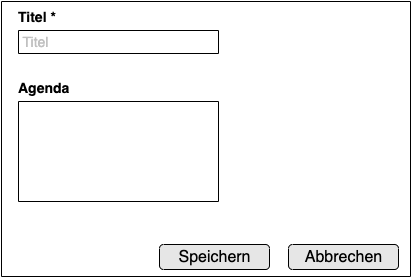
\includegraphics[scale=0.45]{img/workshop_erstellen}
	\caption{Mockup für das Erstellen eines neuen Workshops}  
	\label{fig:workshop erstellen}
  \end{center}   
\end{figure}

Beim Titel des Workshops handelt es sich um ein Linktext. Beim Anklicken wird der Moderator zur \textbf{Controller-Seite} dieses Workshops geführt.
\item Beendete Workshops:\\
Die beendeten Workshops werden in diesem Bereich archiviert. Der Ergebnisse-Button führt zur \textbf{Ergebnisse-Seite} des archivierten Workshops.
\end{enumerate}

\newpage
\subsection{Mockup der Controller-Seite}
\label{subsec:mockup der controller-seite}
Jeder Workshop hat seine eigene Controller-Seite. Die \textbf{Abbildung \ref{fig:controller-seite}} zeigt beispielsweise die Controller-Seite von \glqq Workshops1\grqq{}. Auf dieser sind der Titel des Workshops (Nr.1), die Navigation-Tabs (Nr.2) und die Session-Liste (Nr.3) zu sehen.\bigskip

\begin{figure}[H]
  \begin{center}
    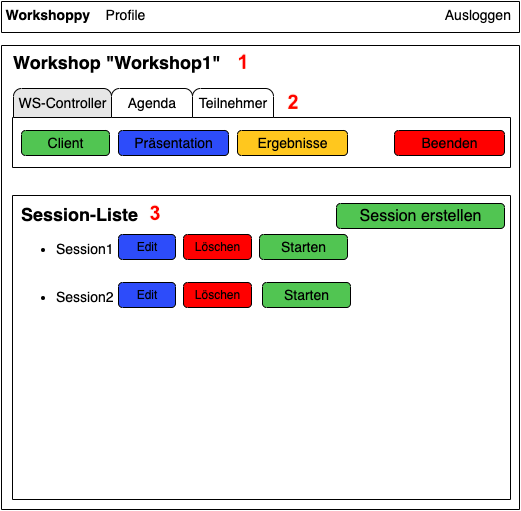
\includegraphics[scale=0.45]{img/controllerseite}
	\caption{Mockup der Controller-Seite}  
	\label{fig:controller-seite}
  \end{center}   
\end{figure}

Es sind drei Navigations-Tabs (Nr.2) vorhanden:
\begin{enumerate}
\item Das Navigation-Tab \glqq WS-Controller\grqq{} beinhaltet vier folgende Buttons:
\begin{itemize}
\item Client-Button:\\
öffnet die \textbf{Teilnehmer-Seite} als neues Browser-Tab. Auf dieser Seite können die Teilnehmer die Dateneingabe tätigen.\\
\textbf{Anmerkung:} Der Client-Button wird in der zukünftigen Weiterentwicklung entfernt, da der Moderator nicht für die Dateneingabe beteiligt werden darf. Für diese Arbeit wird der Client-Button aufgrund des Funktionstests erstmal erhalten bleiben.
\item Präsentation-Button:\\
öffnet als neues Browser-Fenster die \textbf{Präsentation-Seite}. Mittels Beamer präsentiert sie den Teilnehmern die eingegebenen Daten in Echtzeit.
\item Ergebnisse-Button:\\
öffnet ein neues Browser-Tab und ruft die \textbf{Ergebnisse-Seite} auf. Die Ergebnisse des Workshops werden dargestellt. Der Ergebnisse-Button ist erst aktiviert, wenn die Ergebnisse vorhanden sind.
\item Beenden-Button:\\
beendet den laufenden Workshop und leitet den Moderator zur \textbf{Hauptseite} weiter. Der Workshop wird anschließend in \glqq Beendete Workshops\grqq{} archiviert \textbf{(Abbildung \ref{fig:mockup für die hauptseite})}.
\end{itemize}
\item Die Agenda, falls sie vorhanden ist, wird im Navigation-Tab \glqq Agenda\grqq{} dargestellt.
\item Neben dem Einscannen des QR-Codes auf der Präsentation-Seite \textbf{(Abbildung \ref{fig:mockup für das anzeigen des qr-codes})} können die Teilnehmer im Navigation-Tab \glqq Teilnehmer\grqq{} die Einladung per Mail senden lassen, um am Workshop teilzunehmen.\bigskip

\begin{figure}[H]
  \begin{center}
    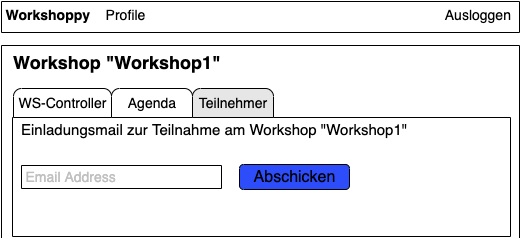
\includegraphics[scale=0.45]{img/einladungsmail}
	\caption{Mockup für das Navigation-Tab \glqq Teilnehmer\grqq{}}  
	\label{fig:mockup für einladungsmail}
  \end{center}   
\end{figure}
\end{enumerate}

Das Brainstorming wird in der Session-Liste (Nr.3) in \textbf{Abbildung \ref{fig:controller-seite}} durchgeführt. Zunächst muss der Moderator mit dem \glqq Session Erstellen\grqq{}-Button eine neue Session anlegen \textbf{(Abbildung \ref{fig:mockup für das erstellen einer neuen session})}.\bigskip

\begin{figure}[H]
  \begin{center}
    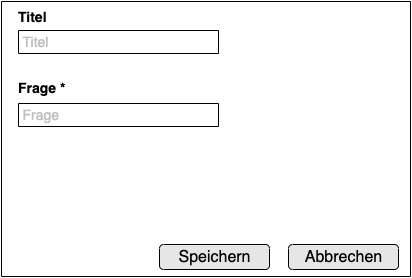
\includegraphics[scale=0.45]{img/session_erstellen}
	\caption{Mockup für das Erstellen einer neuen Session}  
	\label{fig:mockup für das erstellen einer neuen session}
  \end{center}   
\end{figure}

Die behandelte Frage, die auf der \textbf{Teilnehmer- und Präsentation-Seite} zu sehen sein wird, muss definiert werden. Als Option kann der Titel der Session angegeben werden. Wie viele Sessions in einem Workshop benötigt werden, das entscheidet der Moderator selbst. Er kann unbegrenzt viele Sessions erstellen.

\newpage
Neben jeder Session sind in \textbf{Abbildung \ref{fig:controller-seite}} drei Buttons zu sehen. 
\begin{enumerate}
\item Edit-Button:\\
Mit diesem Button kann die Titel- sowie Fragenänderung durchgeführt werden.
\item Löschen-Button:\\
Der Löschen-Button löscht die Session inklusive ihrer zugehörigen Daten.
\item Starten-Button:\\
Es wird erst \glqq gebrainstormt\grqq{}, wenn die Session gestartet ist. Während die Session läuft, darf sie nicht bearbeitet und gelöscht werden. Alle Buttons von nicht aktiven Sessions werden auch in dieser Phase deaktiviert. Es kann nur eine Session gestartet werden. Außerdem kann der Workshop bei laufender Session nicht beendet werden. Der \glqq Beenden\grqq{}-Button in WS-Controller \textbf{(Abbildung \ref{fig:mockup für die aktive session})} wird deshalb deaktiviert.\bigskip

Es gibt zusätzlich noch zwei weiteren Buttons, welche erst sichtbar werden, wenn eine Session gerade läuft. Das ist der \glqq Eingabe beenden\grqq{}- und \glqq Session Beenden\grqq{}-Button \textbf{(Abbildung \ref{fig:mockup für die aktive session})}.

\begin{figure}[H]
  \begin{center}
    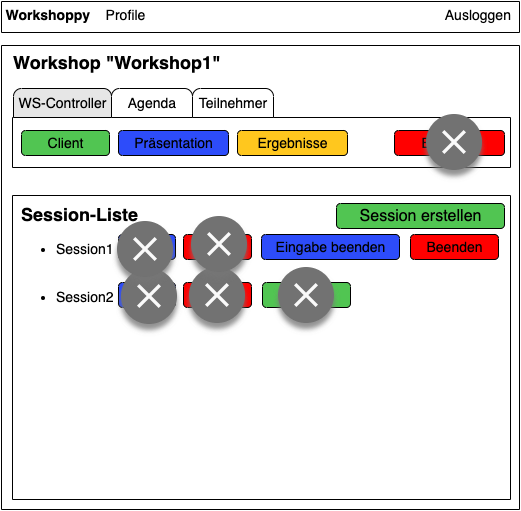
\includegraphics[scale=0.45]{img/session_ist_gestartet}
	\caption{Mockup für die aktive Session}  
	\label{fig:mockup für die aktive session}
  \end{center}   
\end{figure}

Der \glqq Eingabe beenden\grqq{}-Button bricht die Eingabefunktion auf der Teilnehmer-Seite \textbf{(Abschnitt \ref{subsec:Mockup der Teilnehmer-Seite})} ab. Demzufolge können die Teilnehmer keine weiteren Daten mehr eingeben. Der \glqq Session Beenden\grqq{}-Button beendet die gerade laufende Session. Auf der \textbf{Teilnehmer-Seite} wird durch den Klick auf dem \glqq Session Beenden\grqq{}-Button der Infotext \glqq Bitte Warten\grqq{} angezeigt und gleichzeitig wird der QR-Code auf der \textbf{Präsentation-Seite} dargestellt \textbf{(Abbildung \ref{fig:mockup für das anzeigen des qr-codes})}. Erst nach dem Beenden einer laufenden Session werden alle zuvor deaktivierten Buttons wieder reaktiviert.
\end{enumerate}

\subsection{Mockup der Teilnehmer-Seite}
\label{subsec:Mockup der Teilnehmer-Seite}
Um auf diese Seite zu kommen, müssen die Teilnehmer den QR-Code entweder über Ihre Mobilgeräte auf der Präsentation-Seite \textbf{(Abschnitt \ref{subsec:mockup der präsentation-seite})} einscannen oder sie lassen sich per Mail die Einladung zur Teilnahme am Workshop zusenden. Die Teilnehmer-Seite stellt jedem Workshop-Teilnehmer die Dateneingabefunktion zu einer gestarteten Session bereit. Beim Aufrufen der Seite werden die Teilnehmer zunächst aufgefordert, ihren Benutzernamen einzugeben \textbf{(Abbildung \ref{fig:mockup für eingabe der benutzernamen})}.

\begin{figure}[H]
  \begin{center}
    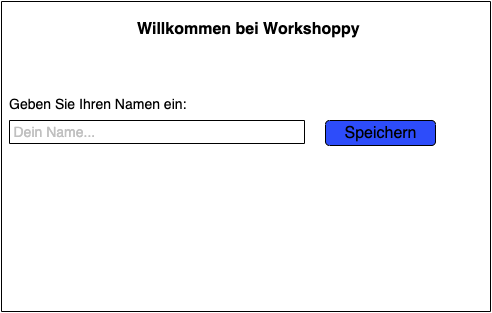
\includegraphics[scale=0.45]{img/teilnehmerseite}
	\caption{Mockup für Eingabe der Benutzernamen}  
	\label{fig:mockup für eingabe der benutzernamen}
  \end{center}   
\end{figure}

Nach Eingabe ihres Benutzernamens werden die Teilnehmer auf die Eingabefunktion weitergeleitet. Die \textbf{Abbildung \ref{fig:mockup für die anzeige der infotext}} beschreibt, dass die Teilnehmer-Seite gerade auf das Kommando des Moderators wartet. Sobald er eine Session startet, werden die Teilnehmer für die Funktionen zur Dateneingabe freigeschaltet \textbf{(Abbildung \ref{fig:mockup für die eingabefunktion})}.

\begin{figure}[H]
	\centering
  \begin{minipage}[t]{0.45\linewidth}
  	    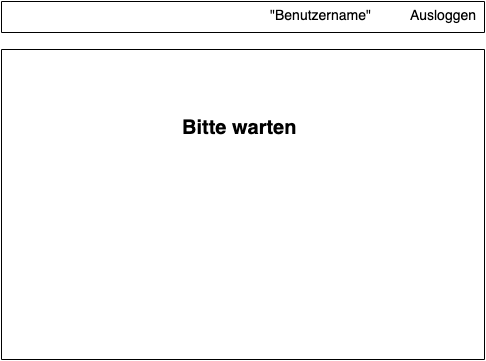
\includegraphics[width=.75\linewidth]{img/teilnehmerseite2}
		\caption{Mockup für die Anzeige der Infotext}
		\label{fig:mockup für die anzeige der infotext}
  \end{minipage}
\hfill
  \begin{minipage}[t]{0.45\linewidth}
    	    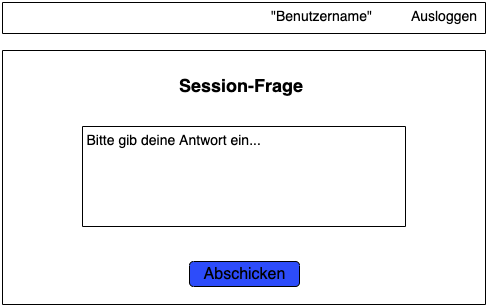
\includegraphics[width=.8\linewidth]{img/teilnehmerseite3}
		\caption{Mockup für die Eingabefunktion}
		\label{fig:mockup für die eingabefunktion}
  \end{minipage}
\end{figure}

In der Navigationsleiste in \textbf{Abbildung \ref{fig:mockup für die anzeige der infotext}} sowie in \textbf{Abbildung \ref{fig:mockup für die eingabefunktion}} sind zwei Navigationselemente zu sehen. Der Benutzername ist der Name des Teilnehmers, welcher zuvor eingegeben wurde. Das Ausloggen erlaubt dem Teilnehmer, seinen Benutzernamen zu ändern. Die Session-Frage in \textbf{Abbildung \ref{fig:mockup für die eingabefunktion}} ist die eigentliche Frage, welche in dieser Session behandelt wird. Die Textarea dient der Dateneingabe. Beim Klick auf den Abschicken-Button wird die Dateneingabe in Echzeit auf der \textbf{Präsentation-Seite} dargestellt.

\subsection{Mockup der Präsentation-Seite}
\label{subsec:mockup der präsentation-seite}
Die Präsentation-Seite dient der Darstellung der Dateneingabe von allen Teilnehmern in Echtzeit. Die Seite hat zwei Zustände, nämlich passiv und aktiv.

\begin{itemize}
\item passiver Zustand:\\
Dieser Zustand bedeutet, dass momentan keine Session läuft. Die Präsentation-Seite zeigt bei diesem Zustand den QR-Code zur Teilnahme am Workshop an. Bevor die Session tatsächlich beginnt, können die Teilnehmer den QR-Code über Ihre Mobilgeräte einscannen, um am Workshop teilzunehmen \textbf{(Abbildung \ref{fig:mockup für das anzeigen des qr-codes})}. Falls es eine Agenda zu dem Workshop gibt, wird sie neben dem QR-Code dargestellt \textbf{(Abbildung \ref{fig:mockup für das anzeigen eines qr-code und einer agenda})}.\bigskip

\begin{figure}[H]
	\centering
  \begin{minipage}[t]{0.45\linewidth}
  	    \includegraphics[width=.8\linewidth]{img/präsentationseite1}
		\caption{Mockup für das Anzeigen eines QR-Codes}
		\label{fig:mockup für das anzeigen des qr-codes}
  \end{minipage}
\hfill
  \begin{minipage}[t]{0.45\linewidth}
    	    \includegraphics[width=.8\linewidth]{img/präsentationseite2}
		\caption{Mockup für das Anzeigen eines QR-Code und einer Agenda}
		\label{fig:mockup für das anzeigen eines qr-code und einer agenda}
  \end{minipage}
\end{figure}

\newpage
\item aktiver Zustand:\\
Die Präsentation-Seite befindet sich im aktiven Zustand, wenn die Session gestartet ist. Auf der Präsentation-Seite werden die Dateneingaben der Teilnehmer in Echtzeit präsentiert \textbf{(Abbildung \ref{fig:mockup für die darstellung der dateneingabe auf der präsentation-seite})}.\bigskip

\begin{figure}[H]
  \begin{center}
    \includegraphics[scale=0.5]{img/präsentationseite3}
	\caption{Mockup für die Darstellung der Dateneingabe auf der Präsentation-Seite}  
	\label{fig:mockup für die darstellung der dateneingabe auf der präsentation-seite}
  \end{center}   
\end{figure}

Die behandelte Frage (Nr.1) ist am oberen Inhaltsbereich zu sehen. Die Eingaben der Teilnehmer (Nr.2) werden wie ein Notizzettel visualisiert. Ein Notizzettel besteht aus zwei Teilen, dem Namen des Teilnehmers und seine Idee. Am unteren Bereich der Präsentation-Seite befinden sich zwei Buttons (Nr.3). Während die Session läuft, kann der QR-Code des Workshops mit dem Drücken des QR-Code-Buttons angezeigt werden. Wenn der QR-Code-Button getätigt wird, wandelt er sich anschließend im \glqq QR-Code ausblenden\grqq{}-Button um. Die Session wird dabei nicht beendet und kann mit dem Drücken des \glqq QR-Code ausblenden\grqq{}-Button wieder auf dem Zustand kommen, wie auf der \textbf{Abbildung \ref{fig:mockup für die darstellung der dateneingabe auf der präsentation-seite}} dargestellt ist. Der QR-Code kann sowohl im passiven Zustand \textbf{(Abbildung \ref{fig:mockup für das anzeigen des qr-codes})} als auch im aktiven Zustand dargestellt werden. Der Vollbild-Button wandelt die Präsentation-Seite in den Vollbildmodus um.\bigskip

Um die eingegebenen Daten auf der Präsentation-Seite zusammenfassen zu können, muss die Ideensammlungsphase beendet werden. Dafür klickt der Moderator auf den \glqq Eingabe beenden\grqq{}-Button auf der Controller-Seite, wie in \textbf{Abbildung \ref{fig:mockup für die aktive session}} zu sehen ist. Daraus folgt, dass auf der \textbf{Teilnehmer-Seite} die Eingabefunktion ausgeblendet und stattdessen der Infotext \glqq Bitte Warten\grqq{} angezeigt wird. Durch den Klick auf den \glqq Eingabe beenden\grqq{}- Button auf der \textbf{Controller-Seite} wird der \glqq Kategorie erstellen\grqq{}-Button auf der Präsentation-Seite freigeschaltet, mit dem der Moderator Kategorien erstellen kann \textbf{(Abbildung \ref{fig:mockup für zusammenfassung-modus auf der präsentation-seite})}.

\begin{figure}[H]
  \begin{center}
    \includegraphics[scale=0.5]{img/präsentationseite4}
	\caption{Mockup für das Zusammenfassen von Daten auf der Präsentation-Seite}  
	\label{fig:mockup für zusammenfassung-modus auf der präsentation-seite}
  \end{center}   
\end{figure}

Direkt auf der Präsentation-Seite kann der Moderator die Daten mit der Drag-\&-Drop-Funktion in Kategorien zusammenfassen. Die Kategorien selbst lassen sich nicht verschieben. Das Löschen einer Kategorie erfolgt mit den Klick auf dem X-Button. Es wird nur die Kategorie gelöscht, d.h. die darin befindlichen Daten bleiben auf der Präsentation-Seite erhalten.
\end{itemize}

\subsection{Mockup der Ergebnisse-Seite}
\label{subsec:mockup der ergebnisse-seite}
Mit Klick auf den Ergebnisse-Button in \textbf{Abbildung \ref{fig:mockup für die hauptseite}} sowie in \textbf{Abbildung \ref{fig:controller-seite}} wird die Ergebnisse-Seite des Workshops als neues Browser-Tab geöffnet. Auf der Seite befinden sich die Daten inklusive Kategorien des Workshops. Die Ergebnisse-Seite beinhaltet außerdem einen Button, mit dem die Ergebnisse als eine PDF-Datei heruntergeladen werden kann \textbf{(Abbildung \ref{fig:mockup für die darstellung der ergebnisse des workshops})}.

\begin{figure}[H]
  \begin{center}
    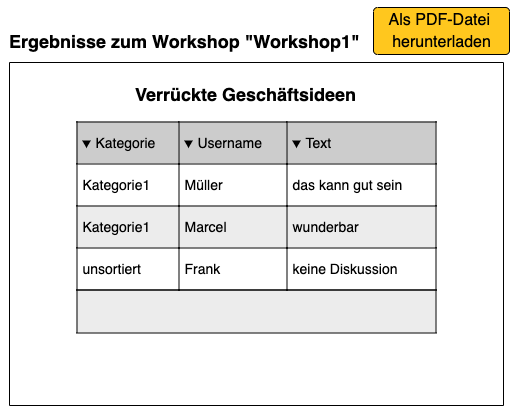
\includegraphics[scale=0.45]{img/ergebnisse_seite}
	\caption{Mockup für die Darstellung der Ergebnisse des Workshops}  
	\label{fig:mockup für die darstellung der ergebnisse des workshops}
  \end{center}   
\end{figure}

\subsection{Zusammenfassung der Konzeption}
\label{subsec:zusammenfassung der konzeption}

\begin{figure}[H]
  \begin{center}
    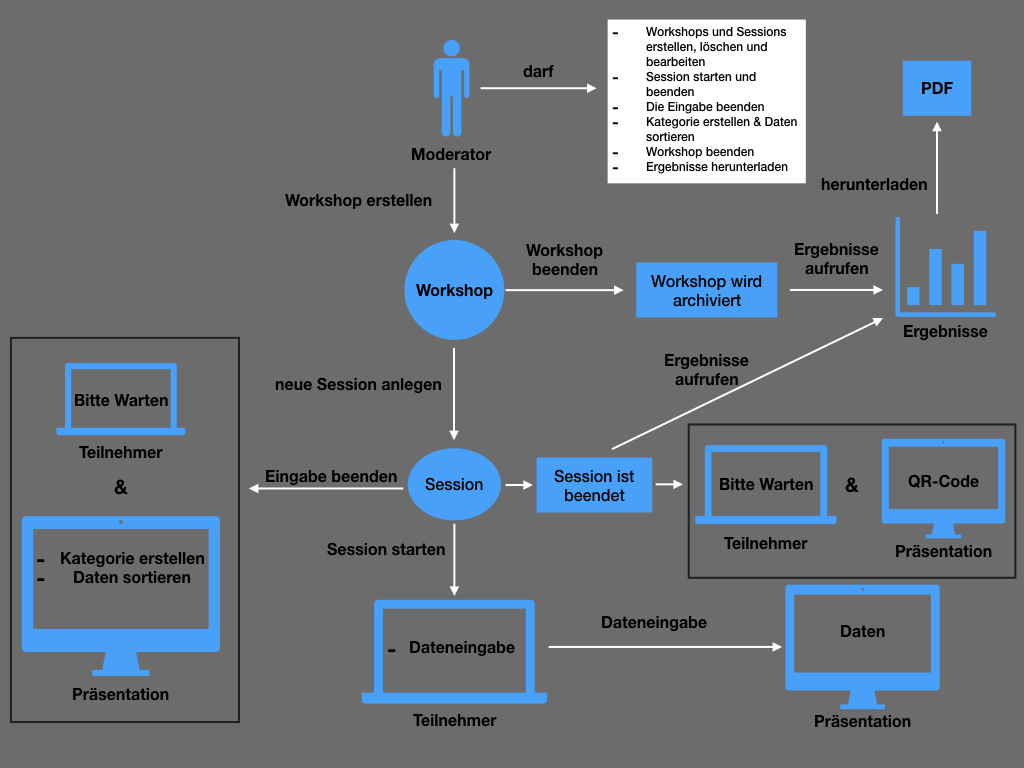
\includegraphics[scale=0.45]{img/Anforderung_neu}
	\caption{Zusammenfassung der Konzeption der zu entwickelnden Webanwendung}  
	\label{fig:zusammenfassung der konzeption}
  \end{center}   
\end{figure}




\chapter{Implementierung}
\label{sec:implementierung}

\chapter{Fazit und Ausblick}
\label{sec:fazit}

%\chapter{Diskussion}
\label{sec:diskussion}

\section{Zusammenfassende Bewertung}
\label{sec:überschrift}

\section{Ausblick}
\label{sec:ausblick}

%Literaturverzeichnis
%\bibliographystyle{unsrt}
\addcontentsline{toc}{chapter}{Literaturverzeichnis}
\bibliographystyle{apalike} 
\bibliography{Literatur}

\end{document}
